\documentclass[12pt,a4paper]{scrartcl}

\usepackage[utf8]{inputenc}
\usepackage[T1]{fontenc}
\usepackage[british,UKenglish,USenglish,american]{babel}

\usepackage{bbm}
\usepackage{hyperref}
\usepackage[pdftex]{graphicx}
\usepackage{graphicx}
\usepackage{latexsym}
\usepackage{amsmath,amssymb,amsthm}
\allowdisplaybreaks
\usepackage{dsfont}
\usepackage{pifont}
\usepackage{nicefrac}
\usepackage{textcomp}
\usepackage{enumitem}
\usepackage{lmodern}


% Abstand obere Blattkante zur Kopfzeile ist 2.54cm - 15mm
\setlength{\topmargin}{-15mm}	   
                  
%\numberwithin{equation}{section} 
\numberwithin{equation}{subsection}

\newcommand{\C}{\mathbb{C}} % komplexe
\newcommand{\R}{\mathbb{R}} % reelle
\newcommand{\Q}{\mathbb{Q}} % rationale
\newcommand{\Z}{\mathbb{Z}} % ganze
\newcommand{\N}{\mathbb{N}} % natuerliche
\newcommand{\PP}{\mathbb{P}} % Probability
\newcommand{\E}{\mathcal{E}} % big Epsilon
\newcommand{\EE}{\mathbb{E}} %Expectation value
\newcommand{\K}{\mathcal{K}}
\newcommand{\1}{\mathbbm{1}}
\newcommand{\G}{\mathcal{G}}
\newcommand{\GG}{\mathfrak{G}}

\numberwithin{equation}{section}

\theoremstyle{definition}
\newtheorem{example}{Example}[subsection]
\newtheorem{theorem}{Theorem}[subsection]
\newtheorem{corollary}{Corollary}[subsection]
\newtheorem{lemma}{Lemma}[subsection]
\newtheorem{definition}{Definition}[subsection]
\newtheorem{proposition}{Proposition}[subsection]
\newtheorem{algorithm}{Algorithm}[subsection]
\newtheorem{prop}{Proposition}[subsection]
\newtheorem{remark}{Remark}[subsection]
\newtheorem{pro}{Proof}
\newtheorem{comment}{Comment}[subsection]


\begin{document}
	\pagestyle{empty}

\begin{titlepage}

	
\includegraphics[scale=0.45]{kit-logo.jpg} 
    \vspace*{2cm} 
\begin{center} \large 
    
   Masterthesis
    \vspace*{2cm}

    {\huge External DLA}\\
    \vspace*{2.5cm}

    Tillmann Tristan Bosch
    \vspace*{1.5cm}

    10. March 2020
    \vspace*{3.5cm}


    Supervisor: PD. Dr. Steffen Winter \\[1cm]
    Faculty of Mathematics\\[1cm]
	Karlsruhe Institute of Technology
\end{center}
\end{titlepage}

\newpage

\newpage
\phantom \\
\newpage

\tableofcontents %Inhaltsverzeichnis

 	\pagestyle{headings}

\setcounter{page}{1}


\newpage

\section{Introduction}
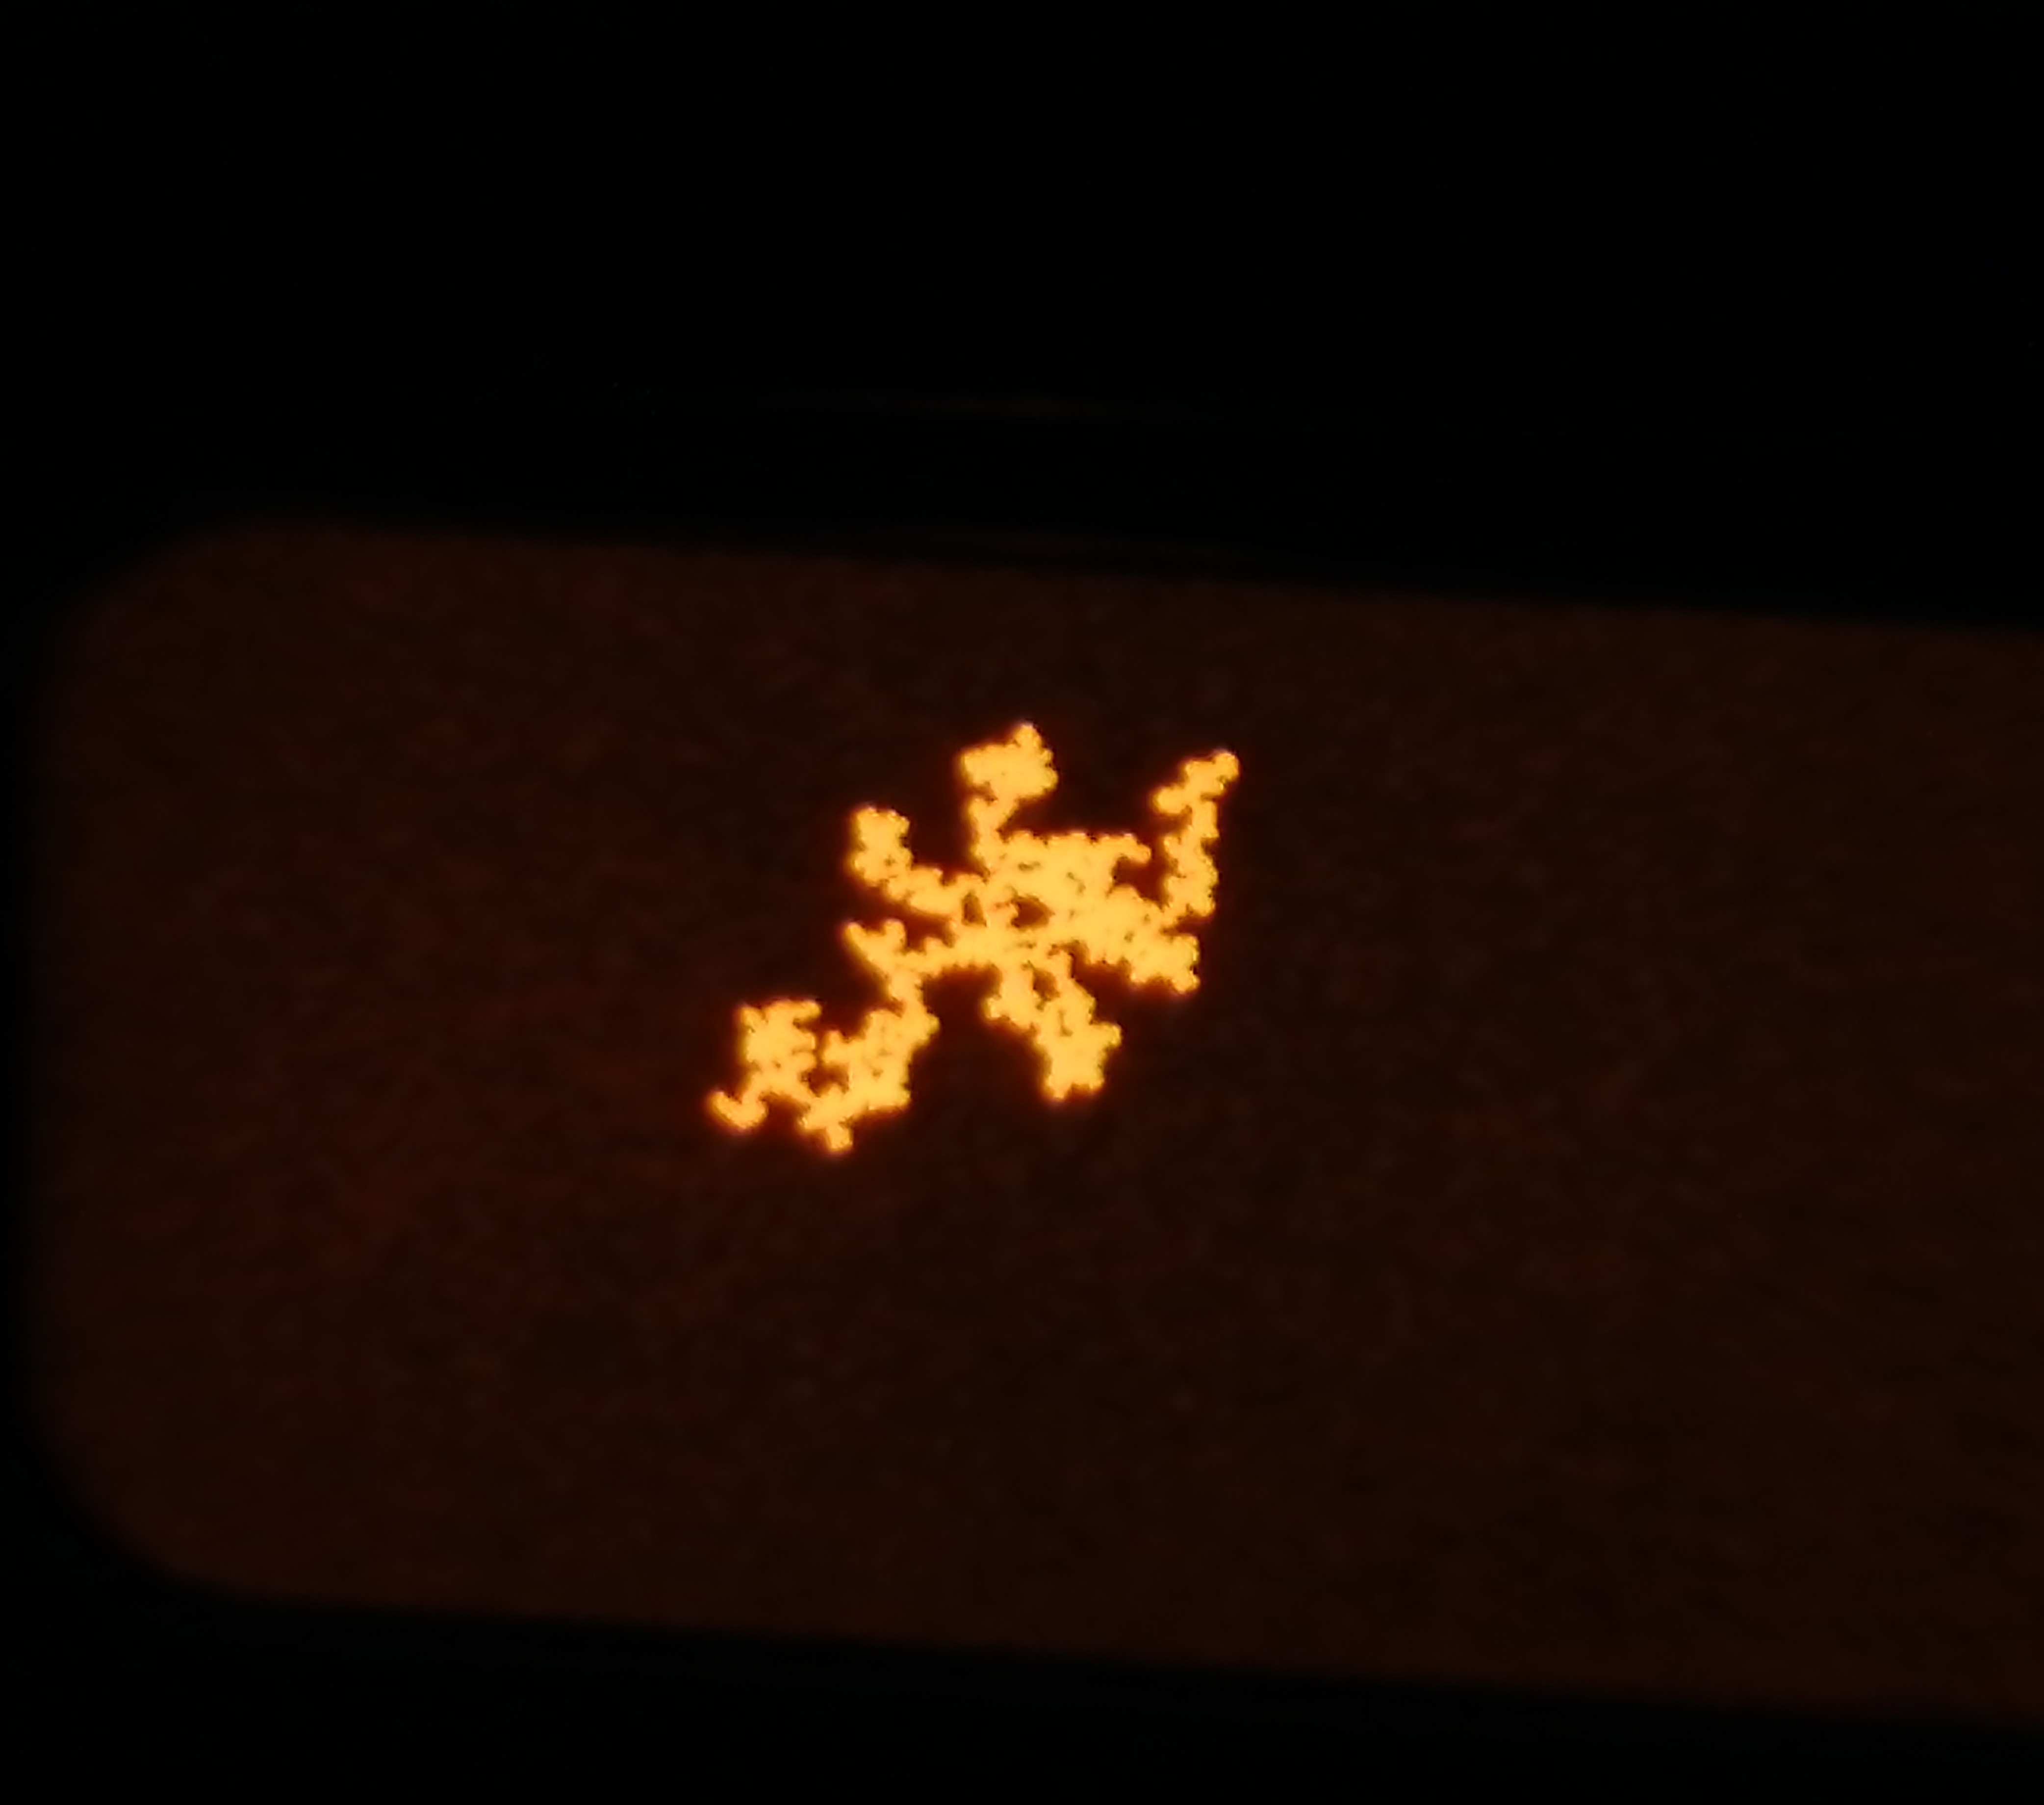
\includegraphics[scale=0.04]{display.jpg} 
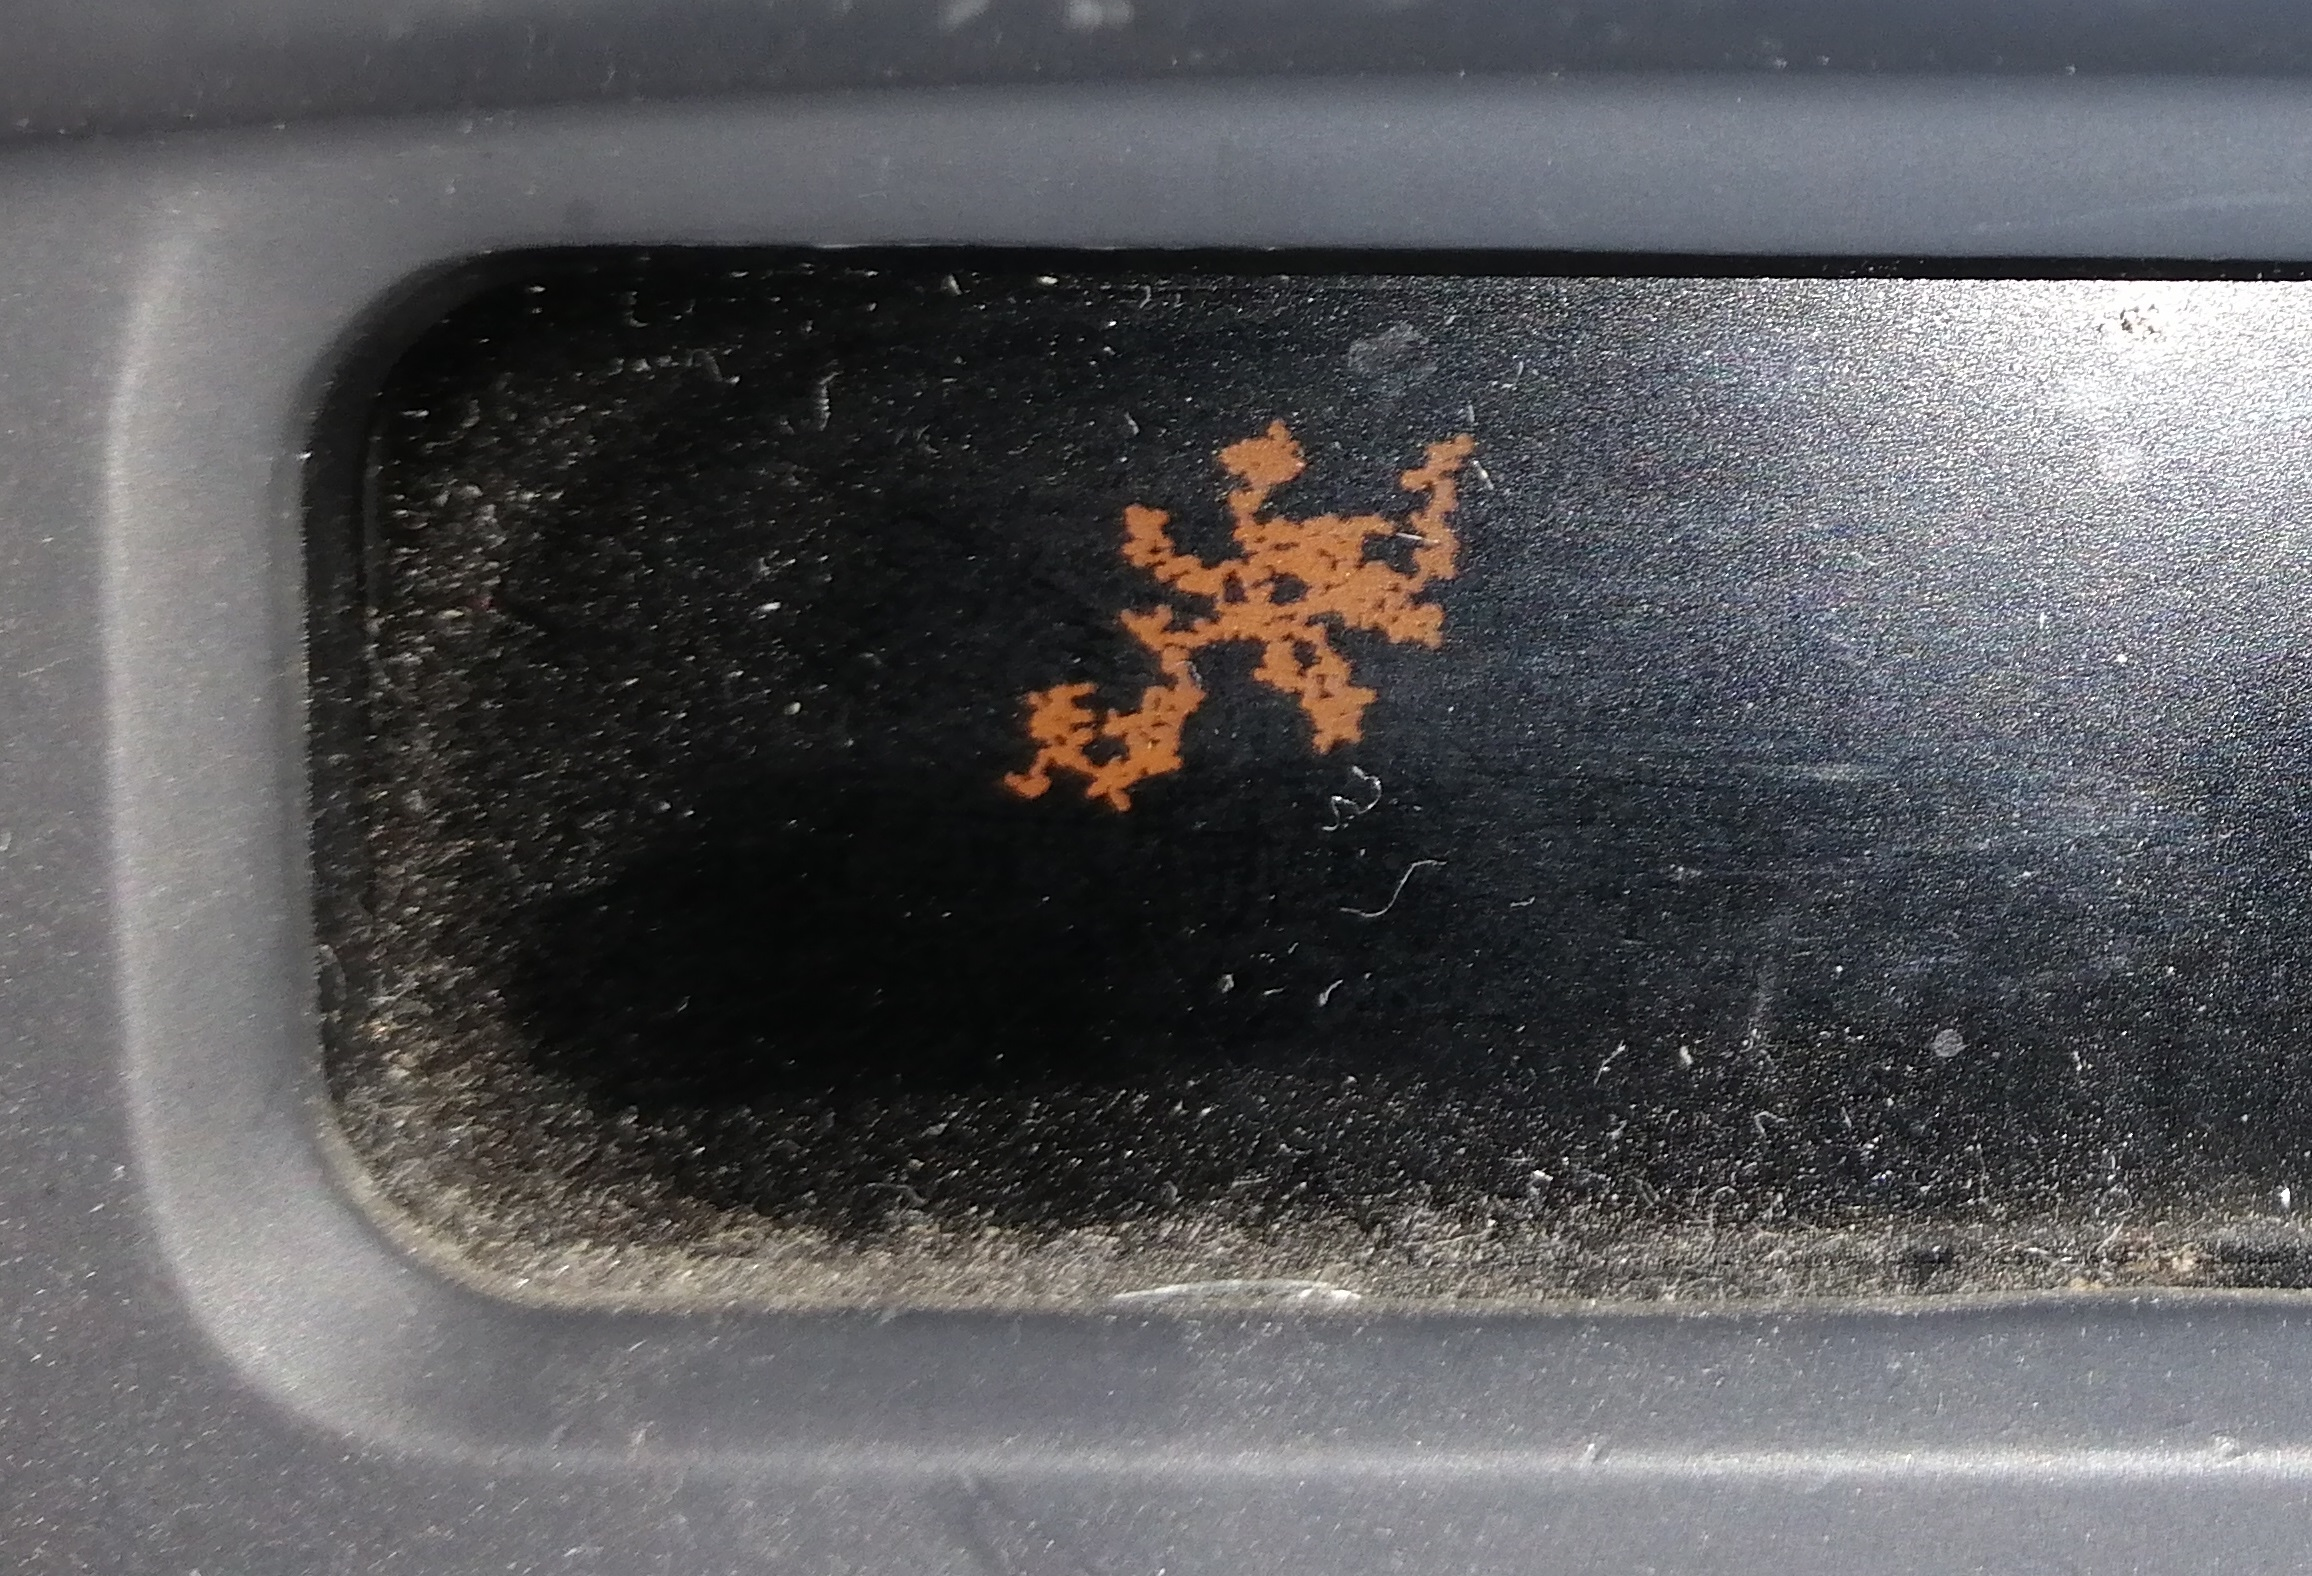
\includegraphics[scale=0.091]{display2.jpg}





\newpage


\section{Preliminaries} \label{prelim}

\subsection{Symbols}
Here we list all Symbols which will be used in this paper. Let $d\in \N$ and $q\in \{0,\dots,d\}$. 
\begin{flalign*}
	&\N = \{1,2,3,\dots\},\quad \text{the set of natural numbers (without 0)}\\
	&\N_0 = \N\cup\{0\}\\
	&\mathcal{B}^d,\quad \text{$d$-dimensional Borel-$\sigma$-algebra of $\R^d$} \\
	&\K^d,\quad \text{the set of convex and compact sets in }\R^d\\
	&B_d(r,x) = \{y\in \R^d\ |\ |x-y| \leq r\},\quad  \text{the $d$-dimensional closed ball of radius $r$ around $x$}\\
	&B_r := B_2(r,0) \\
	&S_{d-1}(r,x) = \partial B_d(r,x),\quad  \text{the $(d-1)$-dimensional surface of the $d$-dimensional ball}\\
	&A(d,q),\quad \text{the set of q-dimensional affine subspaces of }\R^d \\
	&\mathcal{A}(d,q),\quad  \text{the $\sigma$-algebra of } A(d,q), \text{ as constructed later in the paper} \\
	&\G := A(2,1),\quad  \text{the set of lines in the real plane}\\
	&SO_d := \{\nu \in \R^{d\times d}\ |\ \nu \nu^\top = I_d \text{ and } \det \nu = 1\},\quad \text{identify }SO_2 = \{\nu_\beta := e^{i\beta} \in \C\ |\ \beta\in [0,2\pi)\} \\
	&G_d := \{\varphi: \R^d \to \R^d, x\mapsto \nu x+b\ |\ \nu \in SO_d,b\in \R^d\},\quad  \text{the set of euclidean motions} \\
	&\mathcal{P}_f,\quad \text{the set of finite subsets of $\Z^d$ (or $\Z^2$ respective to the context)} \\
\end{flalign*}

\newpage
\subsection{Basic structures}

\subsubsection{Probability Space}

Let $(\Omega,\mathcal{F}, \mathbb{P})$ be a probability space. For our space of interest $\mathbb{Z}^d$ we will always use the discrete $\sigma$-algebra which is the power set of $\mathbb{Z}^d$. If for $A\in \mathcal{F}$ we have $\mathbb{P}(A)=1$ we will say that $\glqq A \text{ holds }\mathbb{P}\text{-a.s.}\grqq$, or short $\glqq A\text{ holds } \text{a.s.}\grqq$ ($A$ holds almost sure). Another short expression, if for a sequence of statements $(A_n)_{n\in\N}$ we say $\glqq$$A_n$ holds for large $n$$\grqq$ it shall mean that for all $M\in\N$ there exists a $n>M$ such that $A_n$ holds. 

\subsubsection{Graphs}

Let $d\in \N$. We will be interested in the undirected graph $(\mathbb{Z}^d, E)$ with its canonical graph structure, which is two vertices (or points) $x=(x_1,\dots,x_d),y=(y_1,\dots,y_d)\in \mathbb{Z}^d$ form an edge (e.q. $\{x,y\}\in E$) if and only if there exists exactly one $i\in \{1,\dots, d\}$ such that $|x_i - y_i| = 1$ and $x_j = y_j$ for all $j\neq i$. For a point $x\in \mathbb{Z}^d$ its set of $\mathit{neighbours}$ is defined as 
\begin{align*}
	N(x) := \{y\in \mathbb{Z}^d\ |\ (x,y)\in E\}.
\end{align*}
For a set $A\subset \mathbb{Z}^d$ the $\mathit{outer\ boundary}\ \partial A$ of $A$ is defined as 
\begin{align*}
	\partial A := \{y\in \mathbb{Z}^d\setminus A\ |\ \exists x\in A:\ (x,y)\in E\}
\end{align*}
Instead of $(\mathbb{Z}^d, E)$ we will write $\mathbb{Z}^d$ from now on. 

\subsubsection{Random Walk}

\begin{definition}
	A family $(S_n)_{n\in \mathbb{N}}$ of measurable functions $S_n: \Omega \to \mathbb{Z}^d$ is called a $\mathit{random\ walk\ on}\ \mathbb{Z}^d$ $\mathit{(starting\ at}\ x\in \mathbb{Z}^d)$ if and only if $S_0=x$ a.s. and 
	
	\begin{align*}
		\mathbb{P}(S_n = y\ |\ S_{n-1} = z) = \frac{1}{|N(z)|} = \frac{1}{2d},\quad \text{ for all }  y\in N(z) \text{ and } z\in \Z^d.
	\end{align*}
	
	\noindent Note that $|N(z)| = 2d$ for all $z\in \mathbb{Z}^d$ since every point has two neighbours in every dimension. We can therefore follow easily that $\mathbb{P}(S_n = y\ |\ S_{n-1} = z) = 0$ for all $y\notin N(z)$ and $z\in \Z^d$. 
\end{definition}
So a Random Walk can be understood as a particle starting from some point $x$ and moving randomly on the grid choosing its next step uniformly from its neighbours. For the following let $(S_n)_{n\in \mathbb{N}}$ be a random walk on $\Z^d$ starting at $x\in \Z^d$. 

\begin{definition}
	Let $A\subset \Z^d$. We define the $hitting\ times$ of A by
	
	\begin{align*}
		T_A := \min \{n\geq 0\ |\ S_n\in A\}\text{ and } T^+_A := \min \{n\geq 1\ |\ S_n\in A\}, 
	\end{align*}
	
	\noindent and $T_y:= T_{\{y\}}$ and $T^+_y:= T^+_{\{y\}}$ for $y\in \Z^d$.
\end{definition}

\begin{definition}
	Define $T:=T^+_x$ to be the first time for the random walk to come back to its origin $x$. The random walk is called $\mathit{recurrent}$ if 
	\begin{flalign*}
		\PP(T<\infty) = 1, 
	\end{flalign*}
	and $\mathit{transient}$ if
	\begin{flalign*}
		\PP(T<\infty) < 1.
	\end{flalign*}
\end{definition}

\begin{lemma} \label{recurr}
	A random walk $(S_n)_{n\in \N}$ on $\Z^d$ is recurrent if $d\leq 2$ and transient if $d\geq 3$. 
\end{lemma}
\begin{proof}
	A detailed proof about this result is presented in $\cite{henze}$ Satz $5.1$. 
\end{proof}

CONTINUE

\begin{definition}
	Now let $d=2$. For $A\subset\Z^2$ define 
	\begin{align*}
		\mathbb{P}_x(S_n\in A) := \mathbb{P}(S_n\in A|S_0=x), \quad n\in\N,x\in\Z^2
	\end{align*}
	and the $heat\ kernel$ of the random walk $(S_n)_{n\in \N}$ as 
	\begin{align*}
		p_n(x,y):=\mathbb{P}_x(S_n=y), \quad n\in\N,x,y\in\Z^2. 
	\end{align*}
	Further define the $\mathit{Green\ function}$ as 
	\begin{align*}
		G(x,y) := \sum_{n\geq 0} p_n(x,y),\quad x,y\Z^2. 
	\end{align*}
	$G$ is well-defined and finite since $\Z^d$ is transient. Similarily for a subset $A\subset \Z^d$ the $killed$ or $\mathit{stopped\ Green\ function}$ is defined as
	\begin{align*}
		G_A(x,y) := \sum_{n\geq 0} \mathbb{P}_x(S_n=y, T_A > n).
	\end{align*} 
\end{definition}


\newpage
\section{Incremental Aggregate}

\subsection{Definition}

In this paper we will look at stochastic processes on the set of finite subsets of $\mathbb{Z}^d$, where we start with a one point set at $\{0\}$ and incrementally add a point on the outer boundary of the current cluster according to some distribution. What we get is a randomly, point by point growing connected cluster which we will call $\mathit{Incremental\ Aggregate}$. Define 
\begin{align}
	\mathcal{P}_f := \{A\subset \mathbb{Z}^d\ |\ \text{A is finite}\}, 
\end{align}
the set of finite subsets of $\mathbb{Z}^d$. Furthermore we will be interested in distributions on those sets, so for $A\in \mathcal{P}_f$ we define 
\begin{align}
	\mathcal{D}_A:= \{\mu: \mathbb{Z}^d\to [0,1]\ |\ \mu(y) = 0 \text{ for all } y\notin A\ \text{and}\ \sum_{y\in A} \mu(y) = 1 \}, 
\end{align}
the set of distributions on $A$. Now we define $\mathit{Incremental\ Aggregate}$ as follows.  

\begin{definition}
	Let $\mu=(\mu_A)_{A\in \mathcal{P}_f}$ be a family of distributions with $\mu_A\in \mathcal{D}_A$ for all $A\in \mathcal{P}_f$. $\mathit{Incremental\ Aggregate\ (with\ distribution\ \mu)}$ is a stochastic process $(\mathcal{E}_n)_{n\in{\mathbb{N}_0}}$ which evolves as follows. The process starts with one point $\mathcal{E}_0 = \{0\}$ at the origin of $\mathbb{Z}^d$. Knowing the process $\mathcal{E}_n$ at time $n$, let $y_n$ be a random point in $\partial \mathcal{E}_n\in \mathcal{P}_f$ with distribution
	\begin{align}
		\mathbb{P}(y_n = y\ |\ \mathcal{E}_n) := \mu_{\partial \mathcal{E}_n}(y),\quad y\in \mathbb{Z}^d.
	\end{align}
	We then define $\mathcal{E}_{n+1} := \mathcal{E}_n \cup \{y_n\}$.
\end{definition} 

For all incremental aggregates in this paper we will focus on the $2$-dimensional case $d=2$. From now on we will identify $\R^2$ with $\C$ as $\R$-vectorspaces. 



\subsection{Notion of Fractal Dimension and Growth Rate}

When there is no strict self-similarity in sets, like in randomly growing clusters as the ones of incremental aggregates, the notion of fractal dimension is not very clear. There are different nonequivalent definitions of what the $\glqq \text{dimension} \grqq$ of a set should be. In many cases they are in fact equivalent and if not it is known in many cases which dimension is bigger than the other one. Here we will mainly consider the following understanding of a dimension of incremental aggregate clusters which we will just call $\mathit{fractal\ dimension}$. This definition is mainly motivated by $\cite{fractalwinter}$ Part II (page 98) and $\cite{lawler}$ 2.6 (page 82). We define the radius of a finite set $A\in \mathcal{P}_f$ as 
\begin{flalign*}
	rad(A) := \max_{x\in A} |x|. 
\end{flalign*}
In a $d$-dimensional ball $B_d(m,0)$ of radius $m$ we could consider a $k$-dimensional subset as a set with cardinality of order $m^k$. Similarly for an incremental aggregate $(\E_n)_{n\in{\mathbb{N}_0}}$ we define the dimension as a value $d_f$ such that 
\begin{flalign*}
	n=|\E_n| \approx \EE[rad(\E_n)]^{d_f}
\end{flalign*}
for large $n$. Formally we can therefore define the fractal dimension as
\begin{flalign} \label{fractaldim}
	d_f := \liminf_{n\to\infty} \frac{ln(n)}{ln(\EE[rad(\E_n)])},
\end{flalign}
if this limit exists. Why choosing $\liminf$ makes sense we will see in the following. The fractal dimension strongly correlates with the growth rate of the aggregate which shall indicate how the radius of the cluster evolves while increasing the particle number. We could express the growth rate by looking for a possibly small exponent $\alpha$ such that there exists a constant $c>0$ with 
\begin{flalign*}
	\EE [rad(\E_n)] \leq cn^\alpha
\end{flalign*}
for large $n$. Rewriting this we come to the equivalent expression
\begin{flalign*}
	\frac{ln(\EE [rad(\E_n)])}{ln(cn)} \leq \alpha
\end{flalign*}
for large $n$ and we could finally define the growth rate $\alpha_f$ of an incremental aggregate as the smallest value holding this expression, so
\begin{flalign} \label{growthrate}
	\alpha_f := \limsup_{n\to\infty} \frac{ln(\EE [rad(\E_n)])}{ln(n)},
\end{flalign}
if the $\limsup$ exists. Since $rad(\E_n) \leq n$ for all $n\in\N$ a.s., this $\limsup$ exists and we get 
\begin{flalign*}
	\alpha_f \leq 1. 
\end{flalign*}
 We further simply have 
\begin{flalign*}
	d_f = \frac{1}{\alpha_f}
\end{flalign*}
and therefore the $\liminf$ in $\ref{fractaldim}$ exists and it is
\begin{flalign*}
	d_f\geq 1.
\end{flalign*}
We will see later how these values behave for incremental aggregates we define in this paper. 



\newpage
\section{External DLA}

\subsection{Definition}

External DLA is a model of an Incremental Aggregate as defined above using a very natural family of distributions, called the $\mathit{harmonic\ measures}$. 

\begin{definition} $\mathit{(Harmonic\ Measure)}$ Let $A\subset\Z^d$. The hitting probability of $A$ is the function 
	\begin{flalign*}
		H_A: \Z^d \times A \to [0,1],\quad (x,y) \mapsto H_A(x,y):=\PP_x(S_{T_A^+} = y).
	\end{flalign*}
	In literature you can find the same definition where $T_A$ is used instead of $T_A^+$. Since in the following for finite sets $A\in\mathcal{P}_f$ the limit $|x| \to \infty$ of $H_A(x,y)$ is of interest, $T_A^+$ is chosen by convenience. In fact for a fixed element $x\in\Z^d$ the function $H_A(x,\cdot)$ defines a measure on $A$ with total mass $\PP_x(T_A^+<\infty)$ and it can be adapted to a probability measure by conditioning the random walk to hit $A$ in finite time. Define
	\begin{flalign*}
		\bar H_A: \Z^d \times A \to [0,1],\quad (x,y) \mapsto \bar H_A(x,y):=\PP_x(S_{T_A^+} = y\ |\ T_A^+<\infty), 
	\end{flalign*} 
	so for fixed $x\in\Z^d$ the function $\bar H_A(x,\cdot)$ defines a probability measure on $A$. Indeed this definition is motivated by $\cite{lawler}\ 2.1$ and in the same chapter it is prooved, that for finite sets $A\in\mathcal{P}_f$ the limit
	\begin{flalign*}
		\lim_{|x|\to\infty} \bar H_A(x,y) =: h_A(y) 
	\end{flalign*}
	exists for each $y\in A$. The function $h_A: A\to [0,1]$ is called the $\mathit{harmonic\ measure\ of\ A}$ and for an element $y\in A$ it displays the probability that a random walk starting at $\glqq \text{infinity}\grqq$ hits $A$ the first time at $y$. If we look at the $2$-dimensional case by Lemma $\autoref{recurr}$ we have that a random walk is recurrent on $\Z^2$ and therefore we get $\bar H_A = H_A$ since $\PP_x(T_A^+<\infty) = 1$ by recurrence. We will call the familiy of distributions $h:=(h_A)_{A\in\mathcal{P}_f}$ $\mathit{harmonic\ measure}$. 
\end{definition}

\begin{definition} $\mathit{(External\ Diffusion\ Limited\ Aggregate)}$ $\mathit{External\ Diffusion\ Limited}$ $\mathit{Aggregate}$, short $\mathit{External\ DLA}$, is an incremental aggregate with the harmonic measure $h$ as distribution. 
\end{definition}


\subsection{Fractal Dimension and Growth Rate of External DLA}

Looking at computer simulations it seems that the clusters of External DLA are formed relatively sparse and they appear to have a noninteger fractal dimension. In $\cite{magnetic}$ DLA is observed in a magnetic aggregation context, and empirically they find a fractal dimension of around $1.8$. Other simulations seem to suggest a value little less than 1.7 for $d_f$ in two dimensions ($\cite{lawler}$ page 83). There is also a theory that predicts 
\begin{flalign*}
	d_f = \frac{d^2 + 1}{d+1}
\end{flalign*}
in $\Z^d$ which seems to agree fairly well with simulations ($\cite{lawler}$ page 83). There are only few rigorously prooved results and one of them we will see in the following. The following theorem and proof are motivated by $\cite{lawler}$ $2.6$. 

\begin{theorem}
	For the growth rate of External DLA in $\Z^2$ according to the definition in $(\ref{growthrate})$ we have
	\begin{flalign}
		\alpha_f \leq \frac{2}{3}. 
	\end{flalign}	
\end{theorem}
\begin{proof}
	To proof this we will show that there exists a constant $c>0$ such that
	\begin{flalign} \label{rad}
		rad(\E_n) \leq cn^{\frac{2}{3}}
	\end{flalign}
	for large $n$ a.s.. Define the bijective function
	\begin{flalign*}
		h: [0,\infty) \to [0,\infty), x\mapsto x^{\frac{2}{3}}. 
	\end{flalign*}
	To show (\ref{rad}) we can also show that there exists a constant $\tilde c>0$ such that 
	\begin{flalign}
		\lambda_n \geq \tilde c h^{-1}(n)
	\end{flalign}
	for large $n$ a.s., where $\lambda_n := \min\{j\in\N\ |\ rad(E_j)\geq n\}$ for $n\in \N$. 
\end{proof}















\newpage
\section{Line Hitting Aggregate}

\subsection{Motivation}

In the following we will look at a process which is the approach of a simple approximation of external DLA on $\mathbb{Z}^2$. The idea is to let particles move on straight lines coming from infinity and add them to the cluster where they hit it. Obviously in most cases particles cannot move completely straight on $\mathbb{Z}^2$. Therefore we will consider points in $\mathbb{Z}^2$ as the centers of unit squares and let the particles move on straight lines in the full plane $\mathbb{R}^2$. We consider a line hitting a point in $\mathbb{Z}^2$ if and only if it intersects with its unit square as defined in the following. 

\begin{definition} \label{squares}
	Define 
	\begin{align}
		\C_{sq} := \{[k - \frac{1}{2}, k + \frac{1}{2}] + [l- \frac{1}{2}, l + \frac{1}{2}]i \subset \C\ |\ k,l \in \mathbb{Z}\}, 
	\end{align} 
	note that $\C = \bigcup_{s\in \C_{sq}} s$. The canonical function
	\begin{align}
	sq: \mathbb{Z}^2 \to \C_{sq},\quad (k,l)\to [k - \frac{1}{2}, k + \frac{1}{2}] + [l- \frac{1}{2}, l + \frac{1}{2}]i
	\end{align}
	is bijective and intuitively identifies points in $\mathbb{Z}^2$ with squares in $\C$ which is $p$ is the center of the square $sq(p)$ for all $p\in \mathbb{Z}^2$. In the following when using a point $p\in \mathbb{Z}^2$ it will reference the point in $\mathbb{Z}^2$ or the corresponding square in $\C$ respecting the context. This bijection also naturally defines a graph structure on $\C_{sq}$, which is two squares $s_1, s_2\in \C_{sq}$ form an edge if and only if $sq^{-1}(s_1)$ and $sq^{-1}(s_2)$ form an edge in $\mathbb{Z}^2$. 
	\noindent For the following we say a line $g$ $hits$ a point $p\in \mathbb{Z}^2$ if and only if $g\ \cap\ sq(p) \neq \emptyset$ (see in $\autoref{linesquares}$). 
	
\end{definition}

\begin{figure}
	\centering
	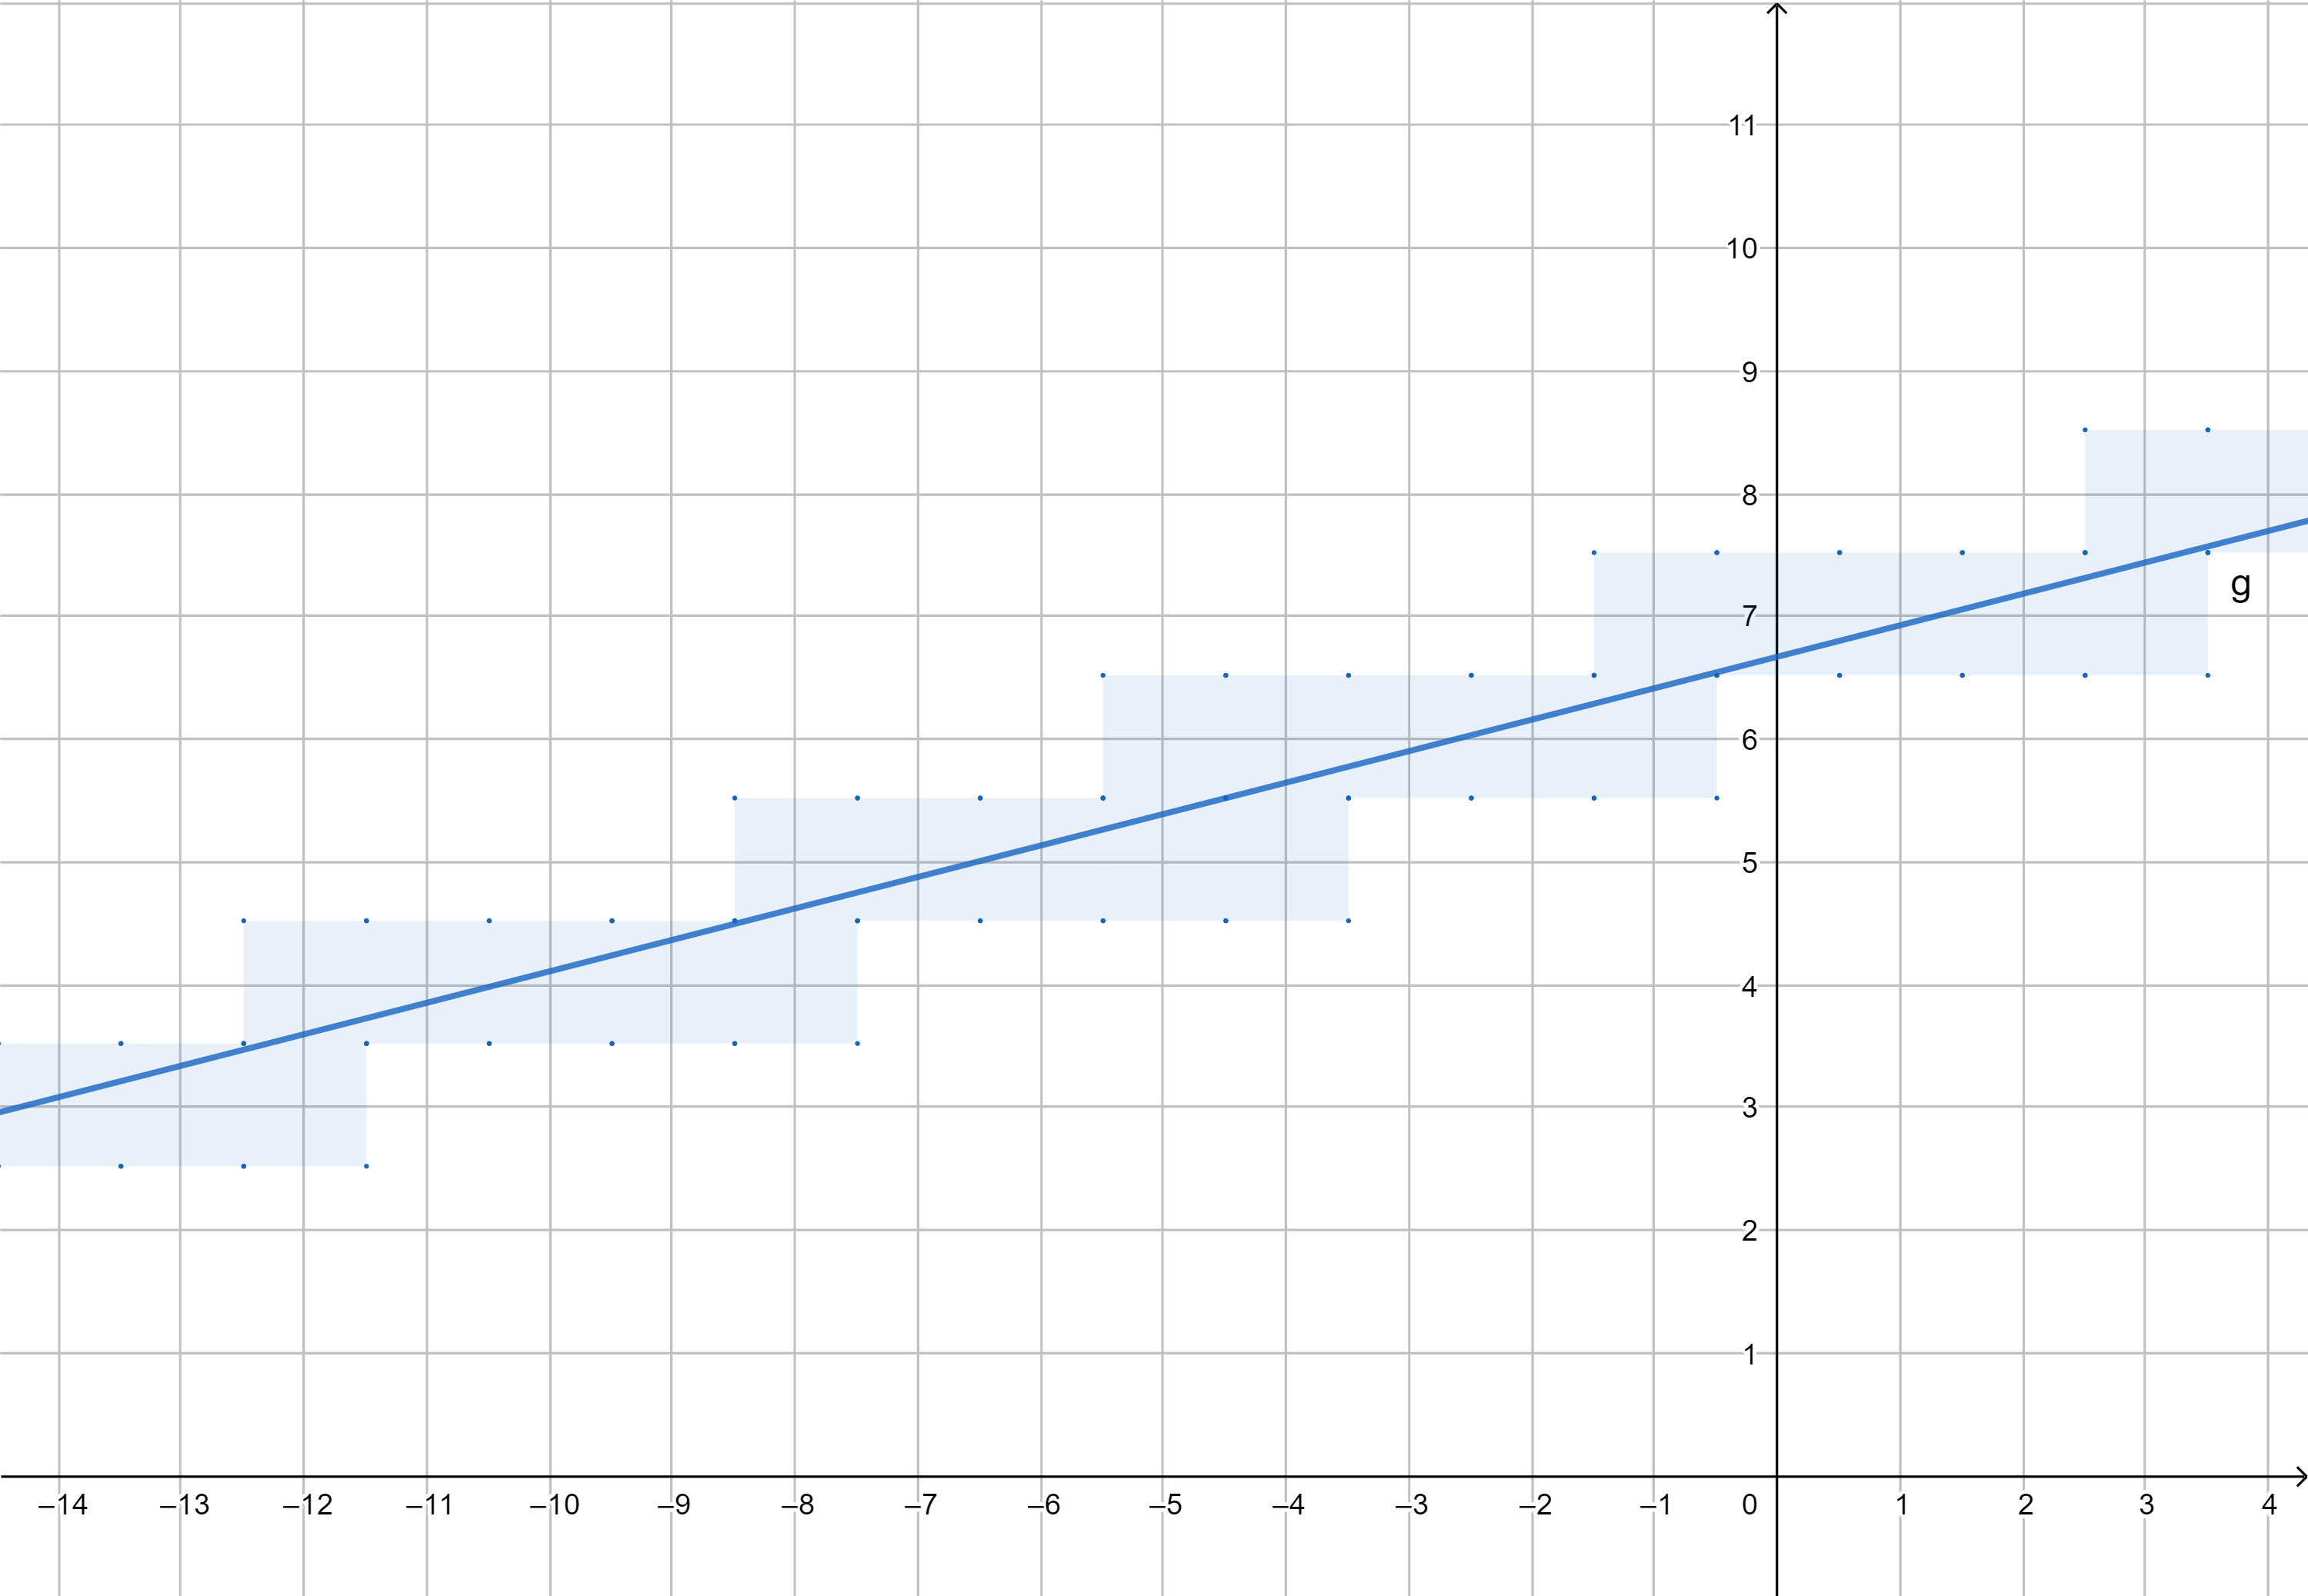
\includegraphics[height=10cm]{line-hit-squares.png}
	\caption{$g$ hits squares around points} \label{linesquares}
	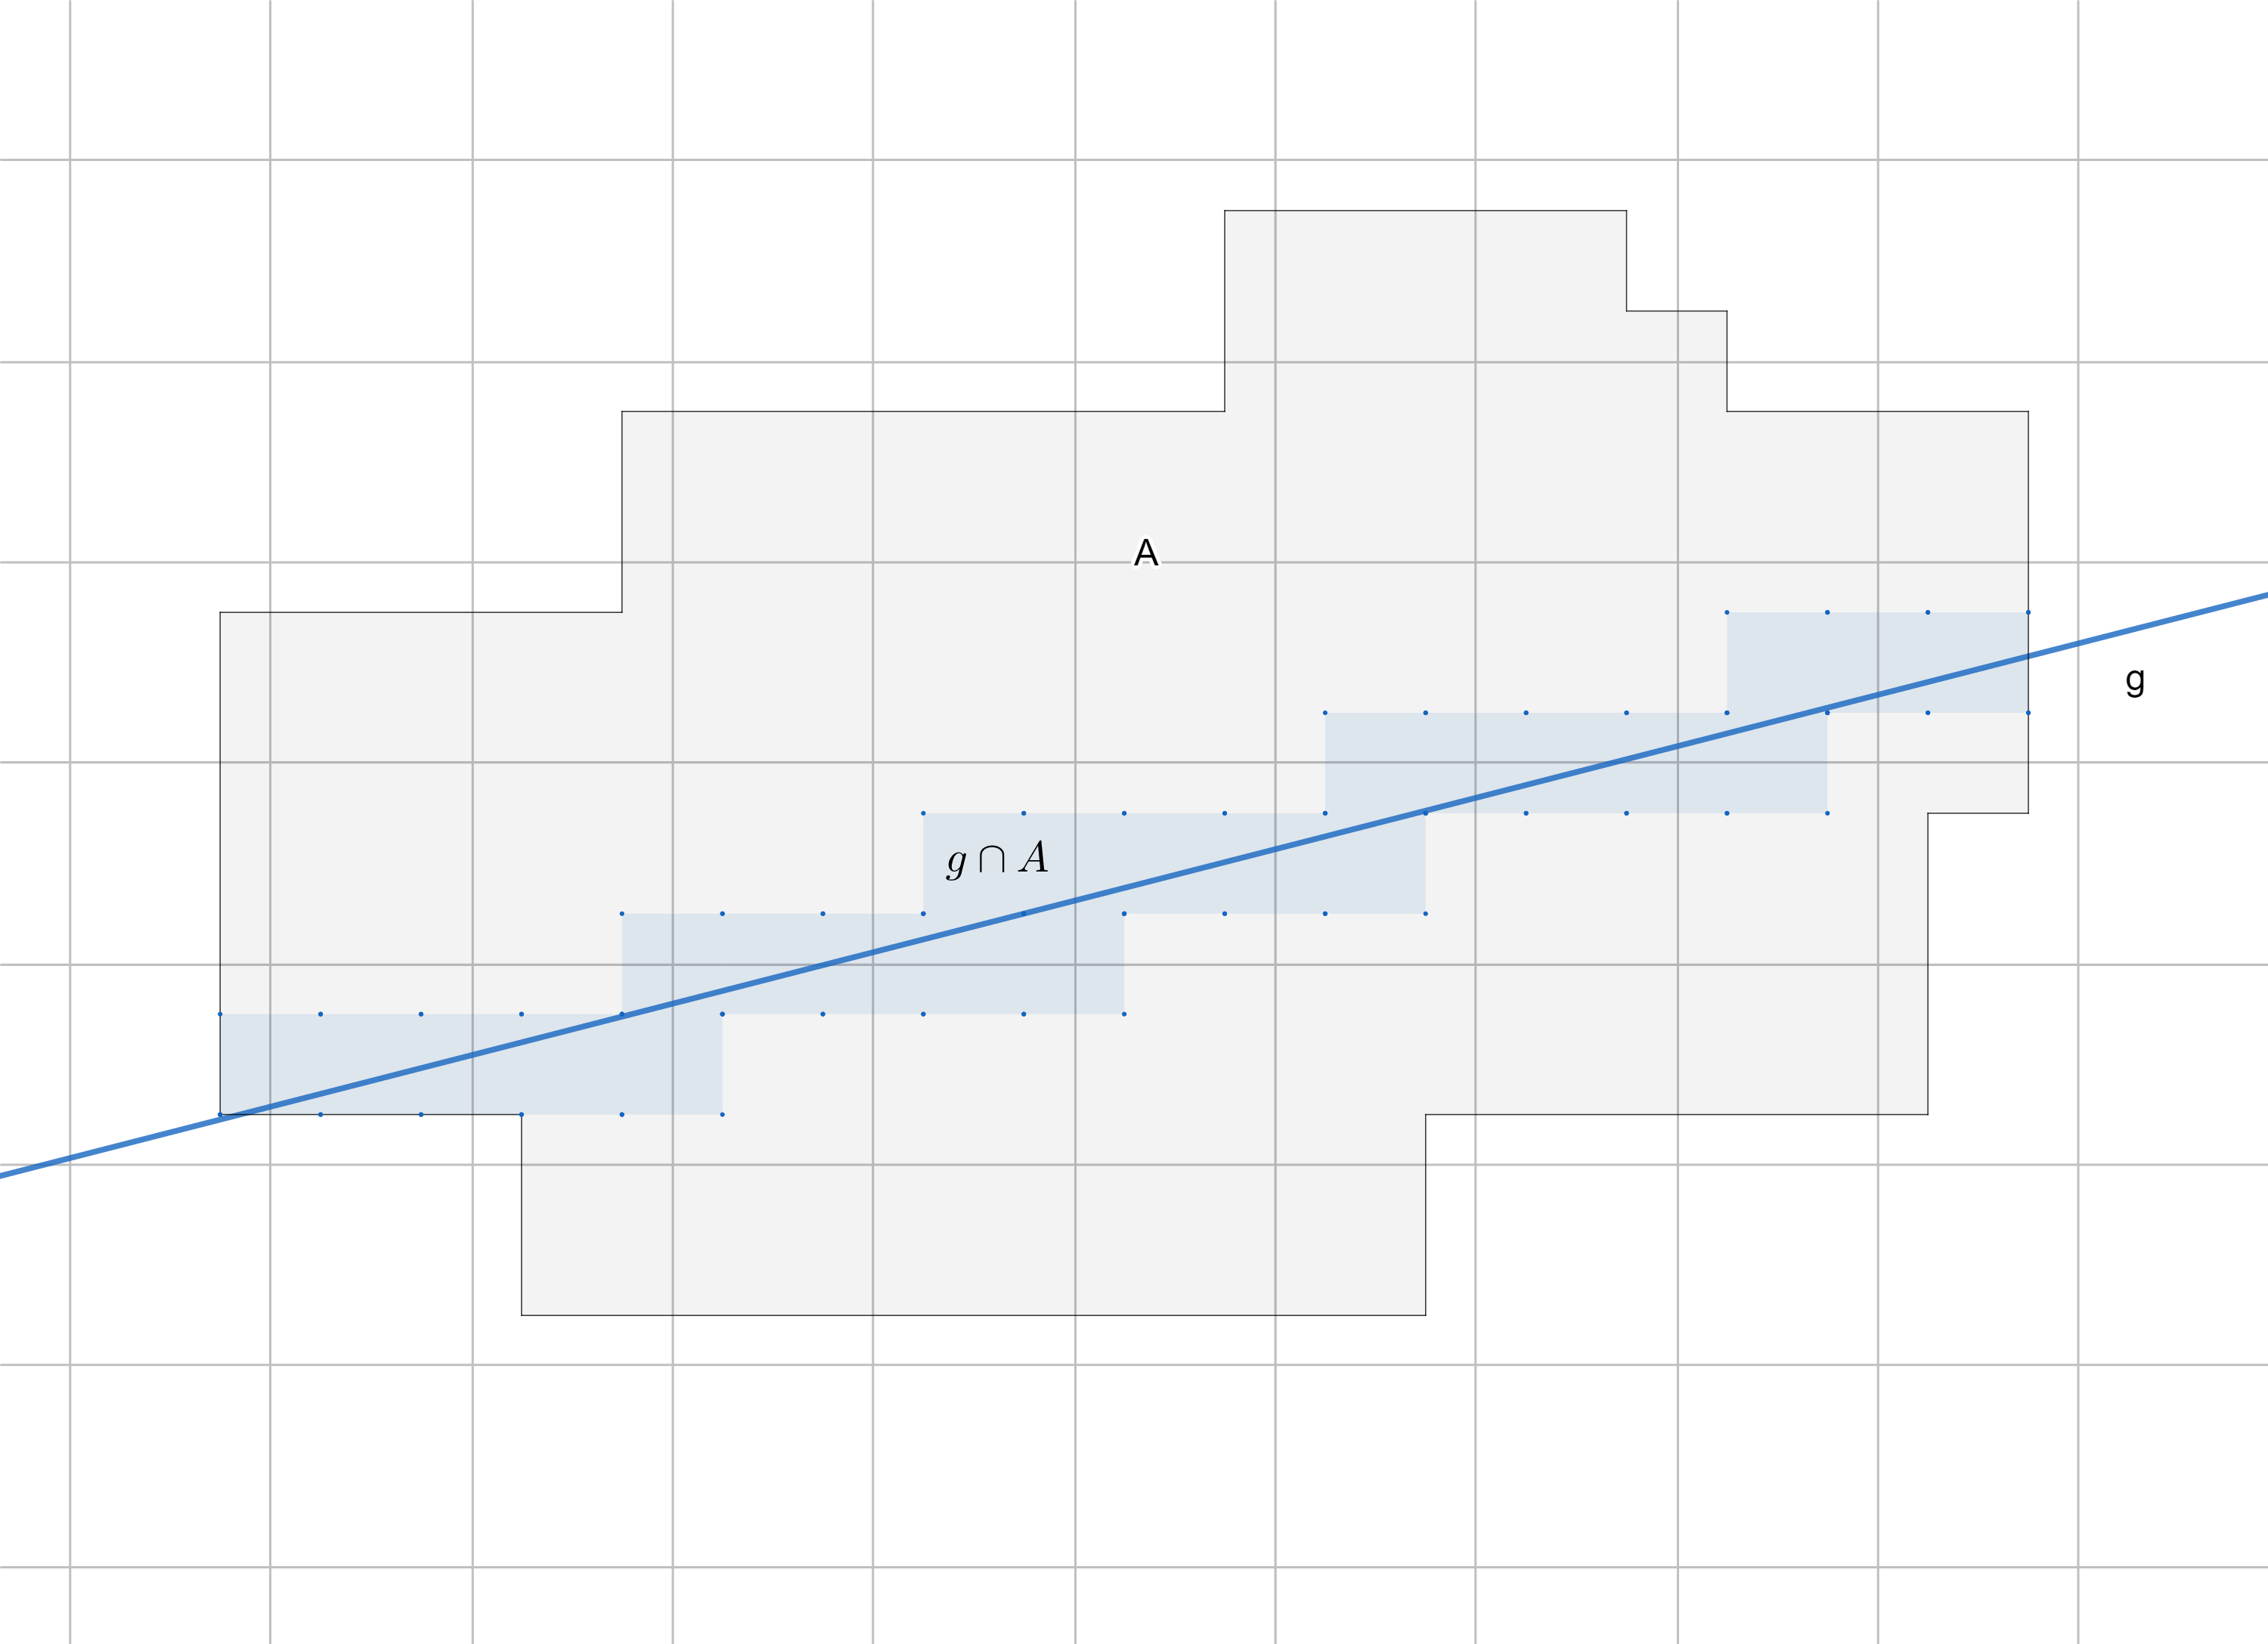
\includegraphics[height=10cm]{line-hit-A.png}
	\caption{$g$ hits squares in $A$} \label{linesquaresA}
\end{figure}

\begin{definition}
	Let $g=g_{\alpha,p}\in \G$ and $A\in \mathcal{P}_f$. We define 
	
	\begin{align*}
		g\cap A := \{ p\in A\ |\ g \text{ hits } p\}
	\end{align*}
	
	which is the subset of all points in $A$ which are hit by $g$ (see $\autoref{linesquaresA}$). For the following we suppose $g\cap A \neq \emptyset$. We will define a total ordered relation $\triangleleft$ on $g\cap A$ which shall be defined equivalently for all $g\in \G$ and $A\in\mathcal{P}_f$ with $g\cap A \neq\emptyset$. We choose two points $x,y\in g\cap A$ and split the definition of the relation $\triangleleft$ into four cases, depending on whether the line $g$ goes from left-bottom to right-top, left-top to right-bottom, parallel to the $x$-axis and parallel to the $y$-axis. Denote the real part of $x$ with $Re(x)$ and the imaginary one with $Im(x)$. \\
	\\
	$\mathit{Case}\ 1:\quad g\ \text{ is parallel to the x-axis}\quad (\Leftrightarrow\quad \alpha = \frac{\pi}{2})$
	\begin{align*}
	x \triangleleft y \quad :\Leftrightarrow \quad Re(x) < Re(y)
	\end{align*}\\
	$\mathit{Case}\ 2:\quad g\ \text{ is parallel to the y-axis}\quad (\Leftrightarrow\quad \alpha = 0)$
	\begin{align*}
	x \triangleleft y \quad :\Leftrightarrow \quad Im(x) < Im(y)
	\end{align*}\\
	$\mathit{Case}\ 3:\quad g\ \text{ is going from left-bottom to right-top}\quad (\Leftrightarrow\quad \alpha\in (\frac{\pi}{2},\pi))$
	\begin{align*}
	x \triangleleft y \quad :\Leftrightarrow \quad
		\begin{cases}
			Re(x) < Re(y), & \text{ if } Re(x) \neq Re(y), \\
			Im(x) < Im(y), & \text{ if } Re(x) = Re(y).
		\end{cases}
	\end{align*}\\
	$\mathit{Case}\ 4:\quad g\ \text{ is going from left-top to right-bottom}\quad (\Leftrightarrow\quad \alpha\in (0,\frac{\pi}{2}))$
	\begin{align*}
	x \triangleleft y \quad :\Leftrightarrow \quad
	\begin{cases}
	Re(x) < Re(y), & \text{ if } Re(x) \neq Re(y), \\
	Im(x) > Im(y), & \text{ if } Re(x) = Re(y).
	\end{cases}
	\end{align*}\\
	It is easy to see that this relation on $g\cap A$ is well-defined. In the following we will prove that this relation is strictly and totally ordered. 
\end{definition}

\begin{lemma}
For a line $g=g_{\alpha,p}\in\G$ and $A\in \mathcal{P}_f$ with $g\cap A\neq \emptyset$ the relation $\triangleleft$ on $g\cap A$ is totally ordered. 
	\begin{proof}
		We will only proove the case where $g$ is going from left-bottom to right-top, which is $\mathit{Case}\ 3$ of the definition. In this case we have $\alpha\in (\frac{\pi}{2},\pi)$. Note, that the proof for $\mathit{Case\ }4$ will work very similar and in the case of $g$ being parallel to one of the axes ($\mathit{Case\ }1$ or $2$), all properties for a totally ordered relation follow directly from the totally ordered relation $<$ on $\mathbb{R}$. So let $\alpha\in (\frac{\pi}{2},\pi)$. \\
		\\
		$\mathit{Antisymmetry:}$ For antisymmetry let $x \triangleleft y$ and $y \triangleleft x$. Suppose $Re(x)\neq Re(y)$, then $Re(x) < Re(y)$ and $Re(y) < Re(x)$, a contradiction because of the total order $<$ in $\mathbb{R}$. So $Re(x) = Re(y)$. But then we have $Im(x) < Im(y)$ and $Im(y) < Im(x)$ and therefore also $Im(x) = Im(y)$, hence $x=y$. \\
		\\
		$\mathit{Transitivity:}$ For transitivity let $x \triangleleft y$ and $y \triangleleft z$. We find four cases. In case $Re(x) \neq Re(y)$ and $Re(y) \neq Re(z)$ we get $Re(x) < Re(z)$ by transitivity of $<$, hence $x \triangleleft z$. In case $Re(x)\neq Re(y)$ and $Re(y) = Re(z)$ we get $Re(x) < Re(y) = Re(z)$, therefore $x \triangleleft z$. In case $Re(x) = Re(y)$ and $Re(y) \neq Re(z)$ we get $Re(x) = Re(y) < Re(z)$, similar as the last case. In the last case $Re(x) = Re(y) = Re(z)$ we get $Im(x) < Im(y)$ and $Im(y) < Im(z)$ and again by transitivity of $<$ we get $Im(x) < Im(z)$, hence $x \triangleleft z$ again. \\
		\\
		$\mathit{Connexity:}$ Connexity is given since for any two points $x,y\in g\cap A$ we have either $Re(x) \neq Re(y)$ or $Re(x) = Re(y)$ and therefore either $x\triangleleft y$ or $y\triangleleft x$.
	 
	\end{proof}
\end{lemma}

\begin{remark}
	The relation $\triangleleft$ on $g\cap A$ basically orders the hitting points of $g$ with $A$ from left to right (or bottom to top in case of a line parallel to the $y$-axis). This order allows us to identify the outermost hitting points which are the minimum and maximum of $g\cap A$ with respect to $\triangleleft$. To clarify, we define $\min (g\cap A) := x_0$ if and only if $x_0 \triangleleft x$ for all $x\in g\cap A,x\neq x_0$, analogously $\max(g\cap A)$. This means when moving on $g$ facing $A$ coming from infinity this order allows to know where in $A$ the line $g$ hits first when "entering" $A$ and where it hits last when "leaving" $A$. 
\end{remark}

Recall that for a bounded subset $A\subset \C$ the convex hull $conv(A)$ of $A$ is defined to be the smallest convex set containing $A$, formally 
\begin{flalign*}
	conv(A) := \bigcap_{A\subset K\in \K^2} K. 
\end{flalign*}
Note that $conv(A)\in \K^2$ for all bounded subsets $A\subset \C$. For a set $A\in \mathcal{P}_f$ we define 
\begin{flalign*}
	conv(A):=conv(\bigcup_{p\in A} sq(p))
\end{flalign*}
and since $\bigcup_{p\in A} sq(p)$ is a bounded set we have $conv(A)\in \K^2$. 

\begin{definition} $\mathit{(Random\ Line\ Hitting\ Distribution)}$ Let $A\in \mathcal{P}_f$ and $K := conv(A)\in \K^2$. For $x\in\Z^2$ and $g\in \G$ define
	\begin{flalign*}
		\tilde \mu_A(x,g) := (\frac{1}{2}\1\{|g\cap A| \geq 2\} + \1\{|g\cap A| = 1\}) \ \1\{x\in \{\min(g\cap A),\max(g\cap A)\}\}
	\end{flalign*}
	and
	\begin{flalign}
		\mu_A(x) := \frac{1}{\PP^K_\mu([A])} \int_\G \ \tilde \mu_A(x,g) \ \PP^K_\mu(dg).
	\end{flalign}
	We quickly show that $\mu_A\in \mathcal{D}_A$. For all $x\in \Z^2\setminus A$ and $g\in \G$ we have $\tilde \mu_A(x,g) = 0$ and therefore $\mu_A(x) = 0$. Furthermore for all $g\in \G$ we have
	\begin{flalign*}
		\sum_{x\in A} \tilde \mu_A(x,g) = \begin{cases}
			\frac{1}{2}2, \quad &|g\cap A| \geq 2, \\
			1, \quad &|g\cap A| = 1, \\
			0, \quad &|g\cap A| = 0.
		\end{cases} \quad= \1\{g\cap A\neq \emptyset\}
	\end{flalign*} 
	and therefore 
	\begin{flalign*}
		\sum_{x\in A} \mu_A(x) = \frac{1}{\PP^K_\mu([A])}\ \int_\G \1\{g\cap A\neq \emptyset\}\ \PP^K_\mu(dg) = \frac{\PP^K_\mu([A])}{\PP^K_\mu([A])} = 1. 
	\end{flalign*}
	Hence, the family of distributions $(\mu_A)_{A\in \mathcal{P}_f}$ defines an incremental aggregate. 
\end{definition}

\begin{definition} $(\mathit{Line\ Hitting\ Aggregate)}$ An Incremental Aggregate with the Random Line Hitting Distribution we call $\mathit{Line\ Hitting\ Aggregate}$, short $\mathit{LHA}$. 
\end{definition}




\subsection{Integral Geometry}

In the next section we want to define an approximation for External DLA. This approximation will be an incremental aggregate for which distribution definition we need some concepts and results from Integral Geometry which we will discuss and develop in this section. In the process we want to define we will want to choose a random line out of all lines which intersect with the current cluster of the aggregate. This random choosing is not obvious since most of the time the cluster will be strongly non symmetric and it is even less obvious how to actually get a realisation of a random line when simulating with Python. In our case we are looking for a parametrisation of lines in the plane and a reasonable way of choosing parameters randomly. \\

We will introduce a possible solution for this problem first through the abstract and general concepts of integral geometry and later through a simple parametrisation for the case of lines in the plane which goes hand in hand with the general result.

\subsubsection{General results}

In the general context we are in $\R^d$ for $d\in \N$ and consider $q$-dimensional affine subspaces where $q\in \{0,\dots,d\}$, short $q$-flats in $\R^d$. The set of $q$-flats in $\R^d$ is denoted by $A(d,q)$. Later we will be interested in choosing random lines in the real plane (i.e. $1$-flats in $\R^2$). In order to get a probability measure on some set of $q$-flats, we first need a measure and a $\sigma$-algebra on $A(d,q)$ in total. 

\begin{definition}
	For $B\in \mathcal{B}^d$ define 
	\begin{flalign*}
		[B]_{d,q} := \{F\in A(d,q)\ |\ F\cap B \neq\emptyset\}.
	\end{flalign*}
	If the context is clear, we will only write $[B]$ instead of $[B]_{d,q}$. 
\end{definition}

\begin{definition}
	The $\sigma$-algebra $\mathcal{A}(d,q)$ on $A(d,q)$ is defined by
	\begin{flalign*}
		\mathcal{A}(d,q) := \sigma(\{ [K]\ |\ K\in \K^d\}).
	\end{flalign*} 
\end{definition}

\begin{theorem} \label{uniqmeas}
	On $A(d,q)$ there exists a unique $G_d$-invariant Radon measure $\mu_q$ such that
	\begin{flalign}
		\mu_q(A_{B_d(1,0)}) = \kappa_{d-q}, 
	\end{flalign}
	where $\kappa_n := \lambda_n(B_n(1,0))$ is the $n$-dimensional Lebesque meausure of the $n$-dimensional unit ball for $n\in \N$, and $\kappa_0:=1$.
\end{theorem}
\begin{proof}
	\cite{stoch1} Theorem 4.26 \\ \\ MAKE PROOF CLEARER
\end{proof}

\subsubsection{Construction in the plane: Isotropic lines}

For our special case we choose $d=2$ and $q=1$, thus lines in the plane. We denote this set of lines by $\G$. The following construction in this chapter is completely motivated by \cite{sackmann} 2.1.1. Firstly we propose a parametrisation of lines which works as follows. Every line can be uniquely determined by an angle $\alpha\in [0,\pi)$ and a real number $p\in \R$. Let $\langle\cdot,\cdot\rangle$ be the standard scalar product on $\R^2$, respectively used for values in $\C$ as we identify $\R^2$ with $\C$ as $\R$-vectorspaces. Let $e_\alpha := e^{\alpha i} = \cos(\alpha) + \sin(\alpha)i$ and $s_\alpha : = -\sin(\alpha) + \cos(\alpha)i$ be the unit vectors $1$ and $i$ rotated by $\alpha$ counterclockwise. Lets consider the representation $x = \langle x,e_\alpha\rangle e_\alpha + \langle x,s_\alpha\rangle s_\alpha$ for $x\in \C$. Since $e_\alpha$ and $s_\alpha$ form a base of $\C$ as a $\R$-vectorspace, the parameters $\langle x,e_\alpha\rangle$ and $\langle x, s_\alpha\rangle$ are unique for each $x$. It thus is easy to realize that $g_{\alpha,p} := \{x\in \C\ |\ \langle x,e_\alpha\rangle  = p\}$ defines a line (compare with $\autoref{lineparam}$) and that every line has a unique pair of $\alpha$ and $p$ for such a representation. In words, $g_{\alpha,p}$ contains all points which have length $p$ in direction of $e_\alpha$. With $\Phi := [0,\pi) \times \R$ this naturally defines a bijection
\begin{flalign*}
	\chi: \Phi \to \G, \quad (\alpha,p) \mapsto g_{\alpha,p}. 
\end{flalign*}
\\
\begin{figure}
	\centering
	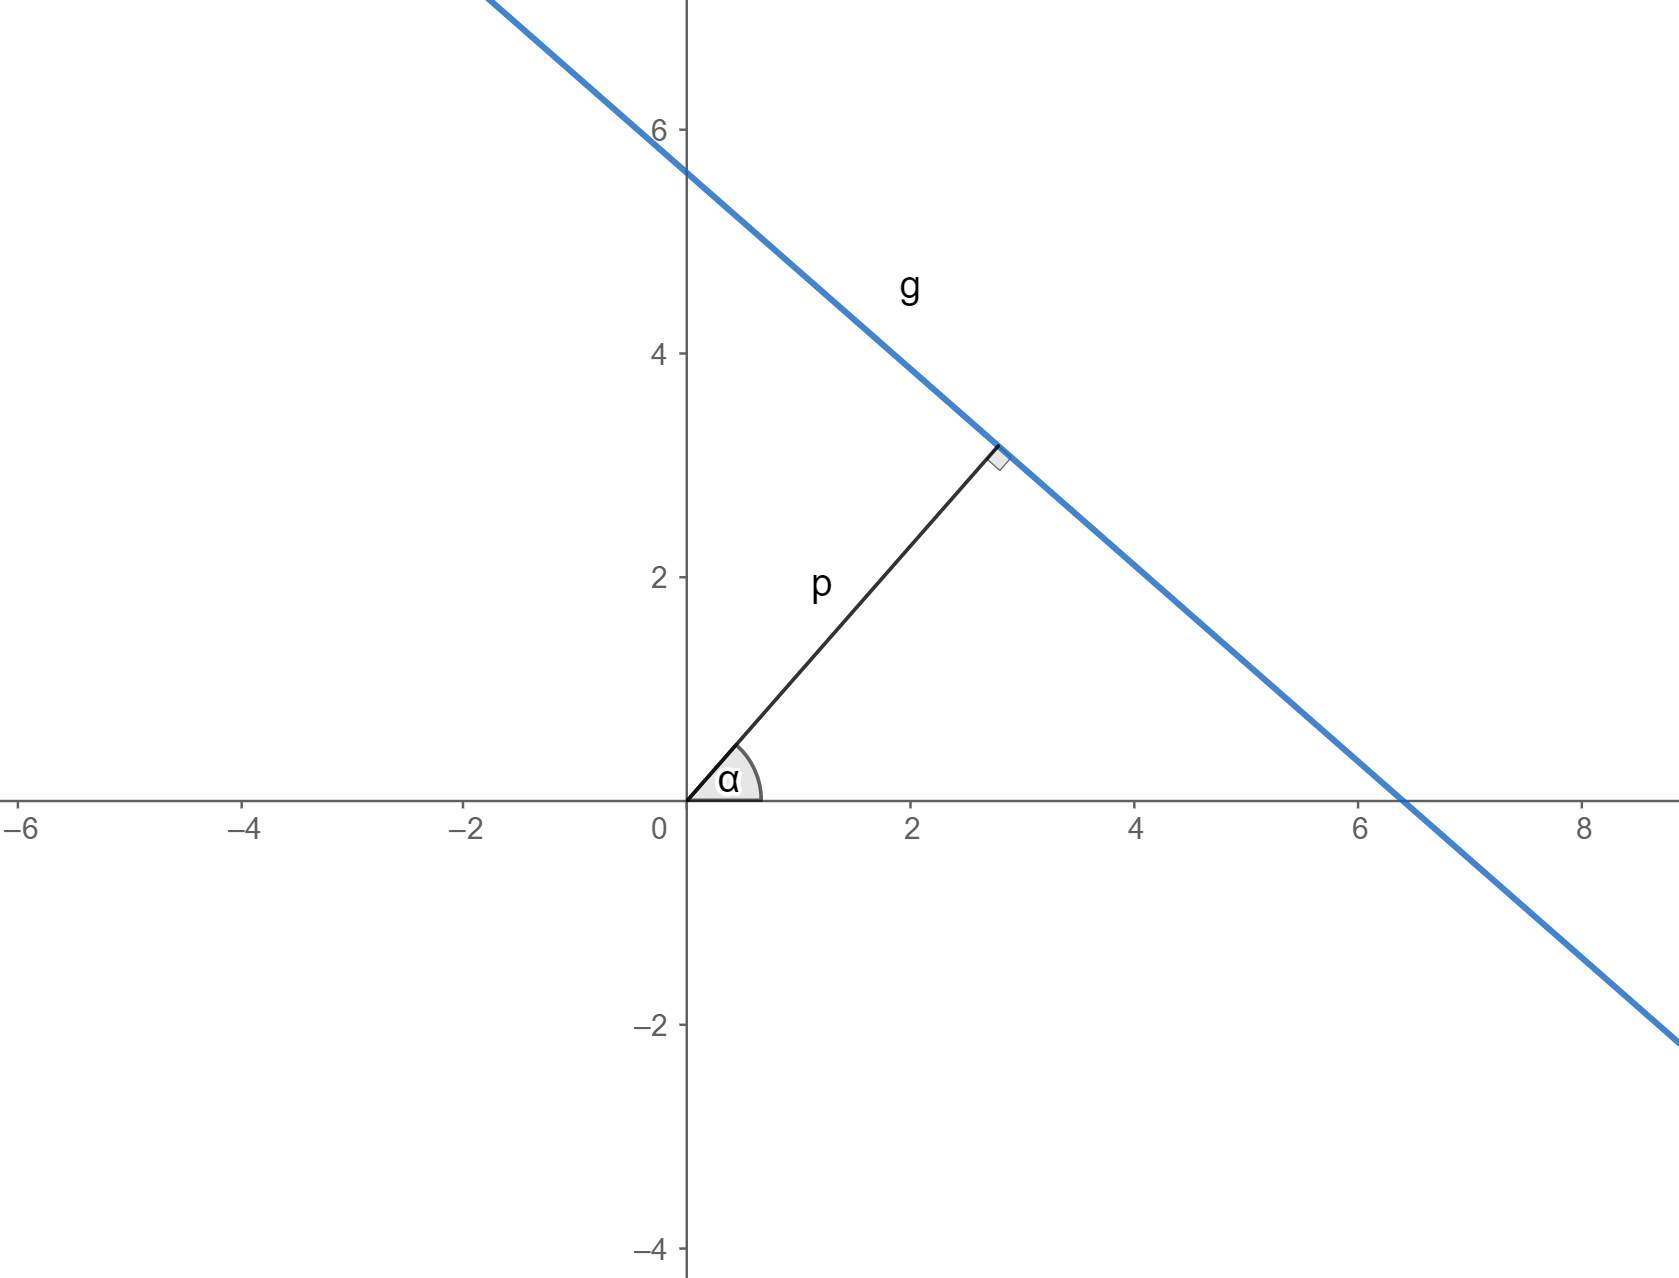
\includegraphics[height=10cm]{line-param.png}
	\caption{Line parameters $\alpha$ and $p$} \label{lineparam}
\end{figure}
\\


We take the subspace Borel-$\sigma$-algebra $\mathcal{B}_\Phi:= \mathcal{B}^2 \cap \Phi$ on $\Phi$ and define the $\sigma$-algebra $\GG$ on $\G$ by $\GG := \chi(\mathcal{B}_\Phi)$. This works well since $\chi$ is a bijection. We want to show in the following that this way of defining a $\sigma$-algebra on $\G$ makes sense as it is indeed equivalent to the general context as defined above. To do that it is convenient to use a special generator set for the Borel-$\sigma$-algebra $\mathcal{B}_\Phi$. 

\begin{lemma} \label{generators}
	Define 
	\begin{flalign*}
		\mathcal{R}_+ := \{[\alpha,\beta]\times (0,b]\ |\ 0\leq \alpha<\beta<\pi, b \geq 0\}, 
	\end{flalign*}
	\begin{flalign*}
		\mathcal{R}_- := \{[\alpha,\beta]\times [b,0)\ |\ 0\leq \alpha<\beta<\pi, b\leq 0\},
	\end{flalign*}
	\begin{flalign*}
		\mathcal{R}_0 := \{[\alpha,\beta]\times \{0\}\ |\ 0\leq \alpha<\beta<\pi\},
	\end{flalign*}
	and
	\begin{flalign*}
		\mathcal{R} := \mathcal{R}_+ \cup \mathcal{R}_- \cup \mathcal{R}_0.
	\end{flalign*}
	Then $\sigma(\mathcal{R}) = \mathcal{B}_\Phi$.
\end{lemma}
\begin{proof}
	We show that $\sigma(\mathcal{R})$ contains all rectangles in $\Phi$ of the form $[\alpha,\beta]\times (a,b]$ with $a,b>0$, $[\alpha,\beta]\times [a,b)$ with $a,b<0$ and $[\alpha,\beta]\times [a,b]$ with $0\in [a,b]$. First let $a,b>0$ and $R=[\alpha,\beta]\times (a,b]$, then 
	\begin{flalign*}
		R = ([\alpha,\beta] \times (0,b]) \setminus ([\alpha,\beta] \times (0,a])
	\end{flalign*}
	and therefore $R\in \sigma(\mathcal{R}_+)\subset\sigma(\mathcal{R})$. Similarly it works if $a,b<0$. If $0\in[a,b]$ then we can write $R = [\alpha,\beta]\times [a,b]$ with three components $R = [\alpha,\beta] \times [a,0) \cup [\alpha,\beta] \times \{0\} \cup [\alpha,\beta] \times (0,b]$ which lie in $\mathcal{R}_-, \mathcal{R}_0$ and $\mathcal{R}_+$ respectively. Therefore $R\in \sigma(\mathcal{R})$ aswell. By measure theory the above described rectangles form a generator set of $\mathcal{B}_\Phi$, which completes the proof. 
\end{proof}

\begin{lemma}
	We have $\mathcal{A}(2,1) = \GG$. 
\end{lemma}
\begin{proof}
	We will consider generators of these $\sigma$-algebras. By Lemma $\autoref{generators}$ we know that $\sigma(\mathcal{R}) = \mathcal{B}_\Phi$ and since $\chi$ is a bijection, we have $\chi(\sigma (\mathcal{R})) = \sigma (\chi(\mathcal{R}))$ and finally $\GG = \sigma(\chi(\mathcal{R}))$. For $\tilde A := \{[K]\ |\ K\in \K^2\}$ we have by definition $\mathcal{A}(2,1) = \sigma(\tilde A)$. \\
	%
	\\ \indent $\subset$: Let $K\in\K^2$. We will show that $\chi^{-1}([K])$ is a closed set in $\Phi$. If that is the case we have $\chi^{-1}([K])\in\mathcal{B}_\Phi$, therefore $[K] \in\chi(\mathcal{B}_\Phi) = \GG$ and finally $\mathcal{A}(2,1) = \sigma(\tilde A)\subset\GG$. To show that $\chi^{-1}([K])$ is closed let $(\alpha_0,p_0)\in \Phi\setminus \chi^{-1}([K])$. Then $\chi(\alpha_0,p_0) \notin [K]$ and therefore $\chi(\alpha_0,p_0) \cap K= \emptyset$. Since $K$ is closed we can find small values $\tilde\alpha,\tilde p > 0$ such that $\chi(\alpha,p) \cap K = \emptyset$ for all $(\alpha,p)\in [\alpha_0, \alpha_0 + \tilde\alpha] \times [p_0, p_0 + \tilde p] =: R$. Hence we have $ R\subset \Phi \setminus \chi^{-1}([K])$, so $\Phi \setminus \chi^{-1}([K])$ is open. Hence $\chi^{-1}([K])$ is closed. \\
	%
	\\ \indent $\supset$: For this inclusion we will show that $\chi(R)\in\mathcal{A}(2,1)$ for all $R\in\mathcal{R}$. First let $R = [\alpha,\beta]\times(0,b]\in\mathcal{R}_+$ for some $b>0$. Define 
	\begin{flalign*}
		S:= \{pe_\gamma \in \C\ |\ (\gamma,p)\in R\}
	\end{flalign*}
	Furthermore for $n\in \N$ define 
	\begin{flalign*}
		A_n := \{tns_\beta\ |\ t\in [0,1]\} \text{ and } B_n := \{-tns_\alpha\ |\ t\in [0,1]\},
	\end{flalign*}
	the segments from $0$ to $ns_\beta$ and $0$ to $-ns_\alpha$ ($\autoref{circleS}$). We will show now that 
	\begin{flalign*}
		\chi(R) = [\bar S] \setminus (\bigcup_{n\in\N} [A_n] \cup \bigcup_{n\in\N} [B_n]) =: \tilde S,  
	\end{flalign*}
	
	\begin{figure}
		\centering
		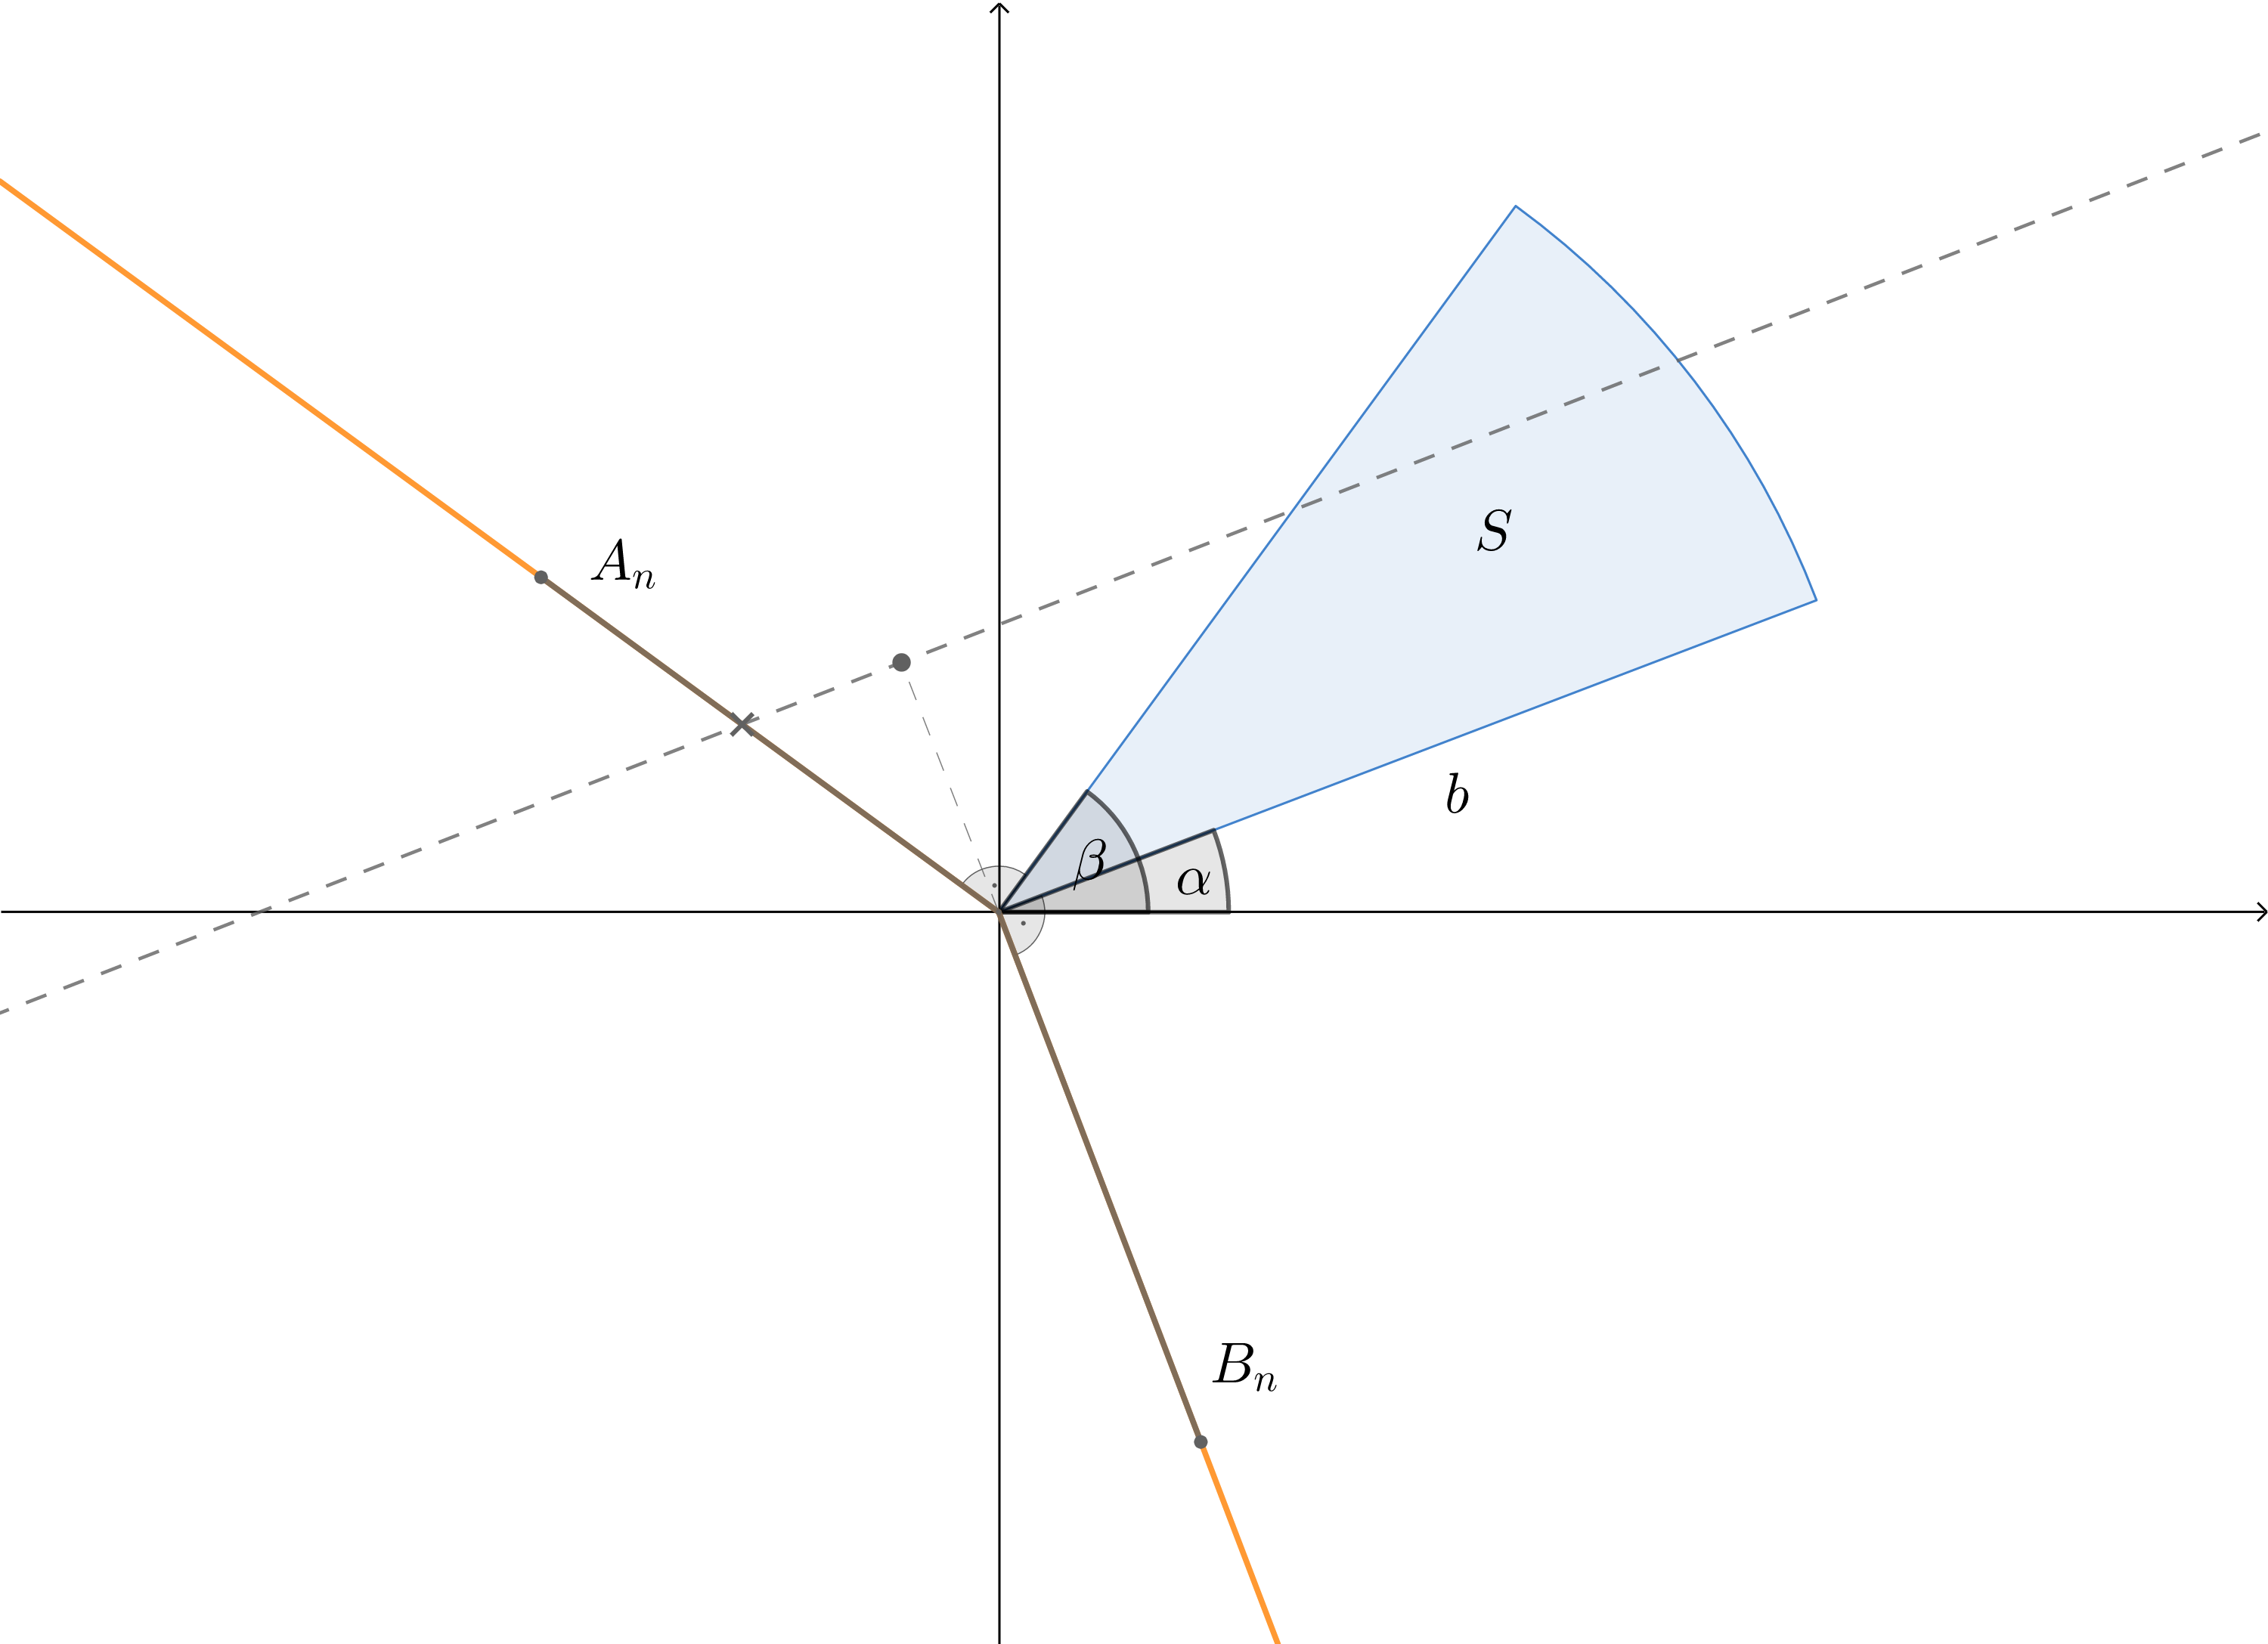
\includegraphics[height=10cm]{circle-part-S.png}
		\caption{$S$ and the sets $A_n$ and $B_n$} \label{circleS}
	\end{figure}
	
	where $\bar S$ is the closure of $S$ (note that $\bar S = S\ \cup\ \{0\}$). Let $(\gamma,p)\in R$. Then $pe_\gamma\in \chi(\gamma,p)\cap S$ and therefore $\chi(\gamma,p)\in [\bar S]$. Assume that there exits an $n\in\N$ such that $\chi(\gamma,p)\cap A_n \neq \emptyset$. Then $\beta + \frac{\pi}{2} - \gamma < \frac{\pi}{2}$, hence $\beta < \gamma$, a contradiction. Similarly argument for any $B_n$, so we finally have $\chi(\gamma,p) \notin [A_n]$ and $\chi(\gamma,p) \notin [B_n]$ for any $n\in \N$. Hence $\chi(\gamma,p)\in\tilde S$ and therefore $\chi(R)\subset \tilde S$. \\
	\\
	Now let $(\gamma,p)\in\Phi$ such that $\chi(\gamma,p)\in \tilde S$. Assume that $\gamma\notin[\alpha,\beta]$ then with a similar argument as in the first inclusion it is easy to see that there must be an $n\in\N$ such that $\chi(\gamma,p)\cap A_n\neq \emptyset$ or $\chi(\gamma,p)\cap B_n\neq \emptyset$, a contradiction. Therefore $\gamma\in[\alpha,\beta]$. Now assume $p\notin (0,b]$. If $p>b$ then $\chi(\gamma,b)\cap B_b = \emptyset$ and since $\bar S\subset B_b$ it is $\chi(\gamma,p)\notin [\bar S]$, a contradiction. If $p<0$ then, since the angle between the segments $A_n$ and $B_n$ opposite of $S$ is strictly smaller than $\pi$, $\chi(\gamma,p)$ must intersect with $A_n$ or $B_n$ for some $n\in\N$, again a contradiction. Note that $p\neq 0$ since $[\{0\}] \subset [A_1]$. Thus we have $p\in(0,b]$. Therefore we have $(\gamma,p)\in R$ and finally $\tilde S\subset \chi(R)$. \\
	\\
	It is left to show that $\tilde S\in \mathcal{A}(2,1)$. All the segments $A_n$ and $B_n$ are compact and convex for all $n\in\N$, and since $S$ is bounded and convex as a circle segment with angle smaller than $\pi$, $\bar S$ is compact and convex. Finally $\tilde S\in \mathcal{A}(2,1)$. \\
	\\
	In total we get $\mathcal{R}_+\subset \mathcal{A}(2,1)$. $\mathcal{R}_-\subset \mathcal{A}(2,1)$ can be shown analogously. So for the last case let $R = [\alpha,\beta] \times \{0\}\in \mathcal{R}_0$. Define the line segment
	\begin{flalign*}
		T := \{(1-t)s_\alpha + ts_\beta\ |\ t\in [0,1]\}. 
	\end{flalign*}
	Then $[\{0\}] \cap [T] \in \mathcal{A}(2,1)$. We show that $\chi(R) = [\{0\}] \cap [T]$. Let $(\gamma,0)\in R$. Then $\chi(\gamma,0)$ contains $0$ and since $\gamma$ is in between $\alpha$ and $\beta$, $\chi(\gamma,0)$ must intersect with $T$ ($\autoref{T}$). For the other inclusion let $(\gamma,p)\in\Phi$ such that $\chi(\gamma,p)\in [\{0\}] \cap [T]$. Since $0\in \chi(\gamma,p)$ it must be $p=0$ and since it intersects with $T$ its angle must lay in between $\alpha$ and $\beta$. All in all this completes the proof. 
\end{proof}

\begin{figure}
	\centering
	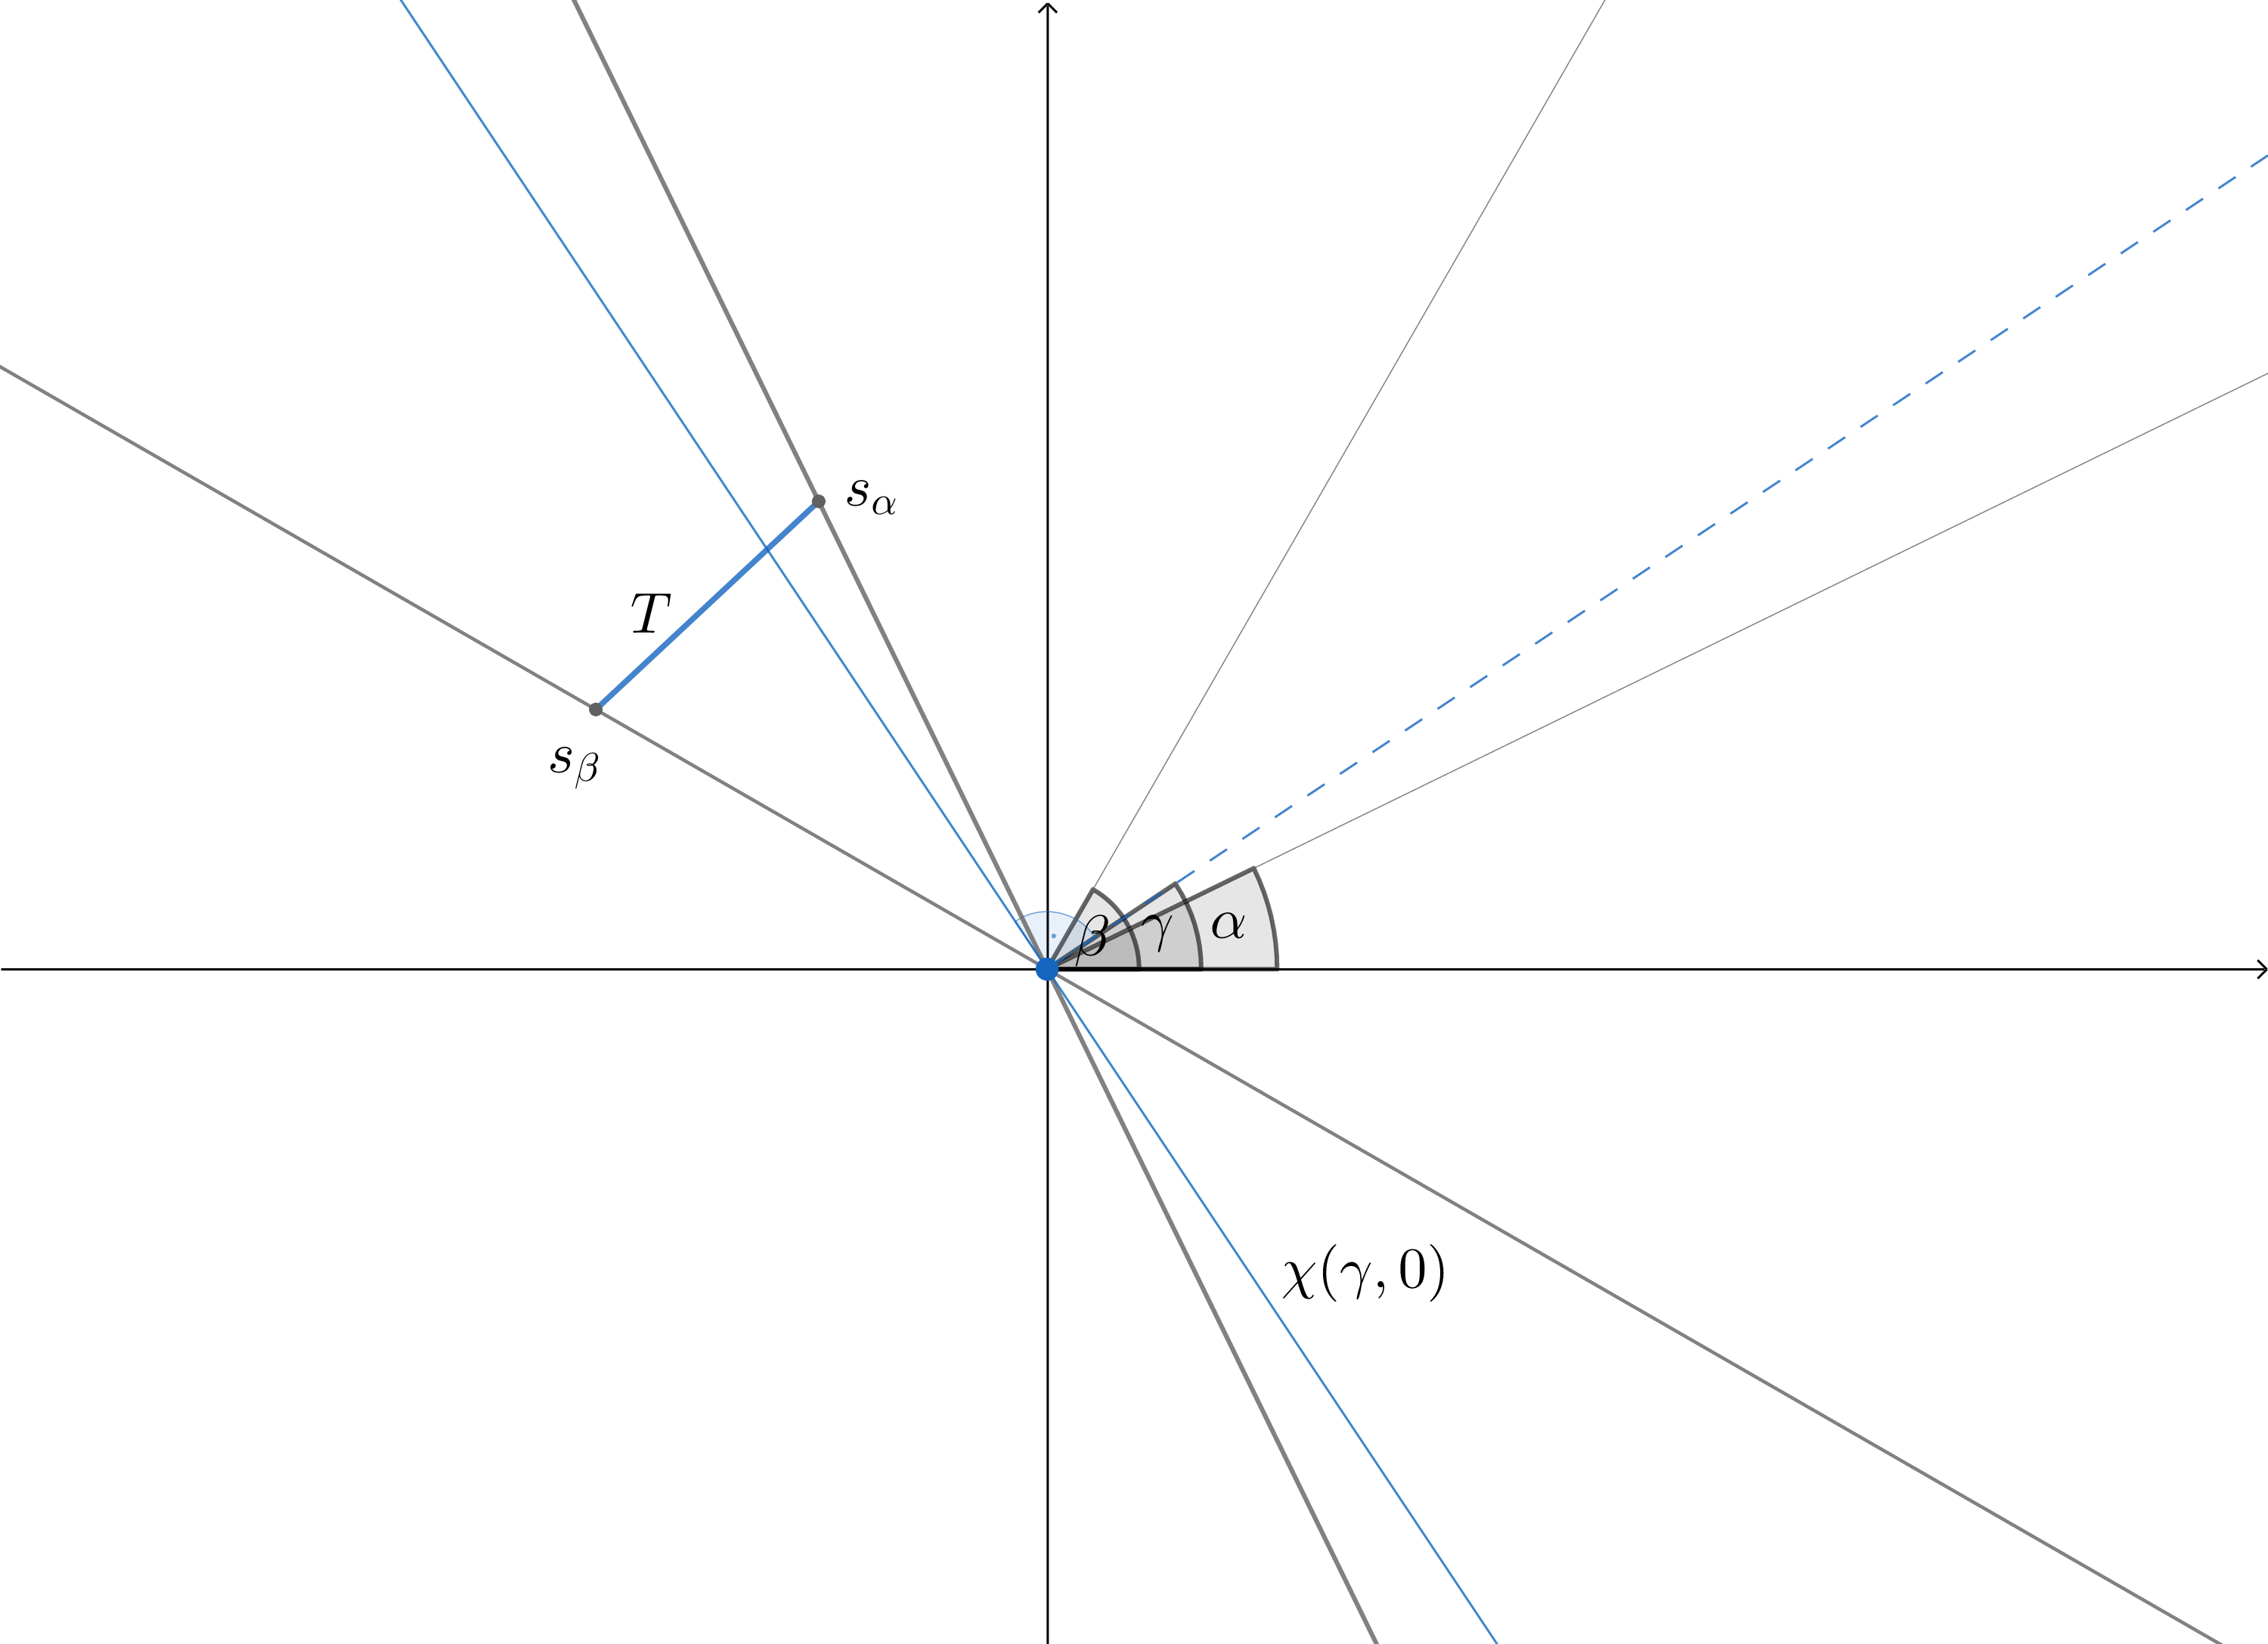
\includegraphics[height=10cm]{T.png}
	\caption{Line in $[\{0\}] \cap [T]$} \label{T}
\end{figure}


\begin{definition}
	A $\mathcal{F}$-$\GG$-measurable function $g:\Omega \to \G$ is called a $\mathit{random\ line}$.  
\end{definition}

\begin{definition}
	We define the measure $\mu := {\lambda_2}_{|\Phi} \circ \chi^{-1}$ on $(\G,\GG)$ where ${\lambda_2}_{|\Phi}$ is the $2$-dimensional Lebesgue measure restricted to $\Phi$. We say a measure $\nu$ on $(\G,\GG)$ is locally finite if for any $K\in \K^2$ we have $\nu([K])<\infty$. 
\end{definition}

\begin{lemma}
	$\mu$ is locally finite and $G_2$-invariant. 
\end{lemma}
\begin{proof}
	Let $K\in \K^2$ and since $K$ is compact choose $r> 0$ such that $K\subset B_r$. Then we have $[K]\subset A_{B_r}$ and
	\begin{flalign*}
		\mu([K]) \leq \mu(A_{B_r}) = {\lambda_2}_{|\Phi} (\chi^{-1}(A_{B_r})) = {\lambda_2}_{|\Phi}([0,\pi)\times [-r,r]) = 2\pi r < \infty, 
	\end{flalign*}
	hence $\mu$ is locally finite. To show that $\mu$ is $G_2$-invariant, that means euclidean motion invariant, we must show it is translation and rotation invariant. First we clarify what exactly translation and rotation mean for lines. We denote $x\ modulo\ r$ as $(x)_r$. For $b\in\C$ and $\beta\in[0,2\pi)$ we define 
	\begin{flalign} \label{motion}
		T_b:\ &\Phi \to \Phi,\quad (\alpha,p) \mapsto (\alpha,p+\langle e_\alpha, b\rangle)
	\end{flalign}
	and
	\begin{flalign} \label{motion2}
		D_{\beta}:\ &\Phi \to \Phi,\quad (\alpha,p) \mapsto ((\alpha + \beta)_{\pi}, \delta((\alpha + \beta)_{2\pi})p), 
	\end{flalign}
	where 
	\begin{flalign*}
		\delta: [0,2\pi) \to \{-1,1\}, \quad \gamma \to \begin{cases}
			1,\ \gamma\in [0,\pi) \\
			-1,\ \gamma\in [\pi,2\pi)
		\end{cases}.
	\end{flalign*}
	It is easy to see that both functions all well-defined. $T_b$ defines a translation by $b$ and $D_\beta$ a rotation by $\beta$. Lets proof that first. Let $(\alpha,p)\in \Phi$, then 
	\begin{flalign*}
		x\in \chi(\alpha,p)+b &\Leftrightarrow x-b\in \chi(\alpha,p) \\ 
		&\Leftrightarrow \langle e_\alpha, x-b\rangle = p \\ 
		&\Leftrightarrow \langle e_\alpha, x\rangle = p + \langle e_\alpha, b\rangle \\
		&\Leftrightarrow x\in \chi(\alpha, p + \langle e_\alpha, b\rangle) \\
		&\Leftrightarrow x\in \chi(T_b(\alpha, p))
	\end{flalign*}
	and therefore $\chi(\alpha,p) + b = \chi(T_b(\alpha, p))$. Hence $T_b(\alpha,p)$ are indeed the parameters for the by $b$ translated line. For the rotation lets devide it into two cases. First let $(\alpha+\beta)_{2\pi} \in [0,\pi)$, then $\delta((\alpha+\beta)_{2\pi}) = 1$ and $(\alpha+\beta)_\pi = \alpha+\beta$ and therefore 
	\begin{flalign*}
		D_\beta(\alpha,p) = (\alpha+\beta,p).
	\end{flalign*} 
	In the second case with $(\alpha+\beta)_{2\pi} \in [\pi,2\pi)$ we have $\delta((\alpha+\beta)_{2\pi}) = -1$ and $(\alpha+\beta)_\pi = \alpha+\beta - \pi$ and therefore
	\begin{flalign*}
		D_\beta(\alpha,p) = (\alpha + \beta - \pi, -p).
	\end{flalign*}
	In the second case we have to carefully understand the parametrisation of $\G$, but finally we can see that $D_\beta(\alpha,p)$ are indeed the parameters of the by $\beta$ rotated line. \\
	\\We will further show now, that $\mu$ is invariant in respect to both these functions. Let $A\in \GG$, $b\in \C$ and $\nu_\beta\in SO_2$ for some $\beta\in[0,2\pi)$. We will understand $A+b = \{g+b\in \G\ |\ g\in A\}$ and $\nu_\beta A = \{\nu_\beta g\in \G\ |\ g\in A\}$ pointwise, and $g+b = \{x+b\ |\ x\in g\}$ and $\nu_\beta g=\{\nu_\beta x\ |\ x\in g\}$ pointwise aswell. We furthermore define $A_p := \{\alpha\in[0,\pi)\ |\ (\alpha,p)\in \chi^{-1}(A)\}$ and $A_\alpha := \{p\in \R\ |\ (\alpha,p)\in \chi^{-1}(A)\}$ for $(\alpha,p)\in \Phi$. For a translation we get 
	\begin{flalign*}
		\mu(A+b) 
		&= \int_\GG \1_{A+b}(g) \mu(dg) \\
		&= \int_\GG \1_A(g-b) \mu(dg) \\
		&= \int_\GG \1_A(g-b) {\lambda_2}_{|\Phi}(\chi^{-1}(dg)) \\
		&= \int_{\chi^{-1}(\GG)} \1_{\chi^{-1}(A)}(\chi^{-1}(g-b)) {\lambda_2}_{|\Phi}(d(\chi^{-1}(g))) \\
		&\overset{(\ref{motion})}{=} \int_\Phi \1_{\chi^{-1}(A)}(\alpha,p-\langle e_\alpha, b\rangle) {\lambda_2}_{|\Phi}(d(\alpha,p)) \\ 
		&= \int_0^\pi \int_\R \1_{A_\alpha}(p-\langle e_\alpha, b\rangle) {\lambda_1}(dp){{\lambda_1}_{|[0,\pi)}}(d\alpha) \\ 
		&= \int_0^\pi \int_\R \1_{A_\alpha +\langle e_\alpha, b\rangle}(p) {\lambda_1}(dp){{\lambda_1}_{|[0,\pi)}}(d\alpha) \\ 
		&= \int_0^\pi \lambda_1(A_\alpha +\langle e_\alpha, b\rangle) {{\lambda_1}_{|[0,\pi)}}(d\alpha) \\ 
		&\overset{(+)}= \int_0^\pi \lambda_1(A_\alpha) {{\lambda_1}_{|[0,\pi)}}(d\alpha) \\ 
		&= \dots \\
		&= \mu(A),
	\end{flalign*}
	and for a rotation we get
	\begin{flalign*}
		\mu(\nu_\beta A) &= \int_\G \1_{\nu_\beta A}(g) \mu(dg) \\
		&= \int_\G \1_A(\nu_{-\beta} g) {\lambda_2}_{|\Phi}(\chi^{-1}(dg))\\
		&= \int_{\chi^{-1}(\G)} \1_{\chi^{-1}(A)}(\chi^{-1}(\nu_{-\beta} g)) {\lambda_2}_{|\Phi}(d(\chi^{-1}(g)))\\
		&\overset{(\ref{motion2})}= \int_\Phi \1_{\chi^{-1}(A)}((\alpha - \beta)_{\pi}, \delta((\alpha - \beta)_{2\pi})p) {\lambda_2}_{|\Phi}(\alpha,p) \\
		&= \int_\Phi \1_{\chi^{-1}(A)}((\alpha - \beta)_{\pi}, \delta((\alpha - \beta)_{2\pi})p) {\lambda_2}_{|\Phi}(\alpha,p) \\
		&= \int_{0}^{2\pi} \int_\R \1_{\chi^{-1}(A)}((\alpha - \beta)_{\pi}, \delta((\alpha - \beta)_{2\pi})p) {\lambda_1}(dp){{\lambda_1}_{|[0,\pi)}}(d\alpha) \\
		&= \int_{0}^{2\pi} \int_\R \1_{A_{(\alpha - \beta)_{\pi}}}(\delta((\alpha - \beta)_{2\pi})p) {\lambda_1}(dp){{\lambda_1}_{|[0,\pi)}}(d\alpha) \\
		&\overset{(+)}= \int_{0}^{2\pi} \int_\R \1_{A_{(\alpha - \beta)_{\pi}}}(p) {\lambda_1}(dp){{\lambda_1}_{|[0,\pi)}}(d\alpha) \\
		&= \int_\R \int_{0}^{2\pi} \1_{\chi^{-1}(A)}((\alpha - \beta)_{\pi}, p) {{\lambda_1}_{|[0,\pi)}}(d\alpha){\lambda_1}(dp) \\
		&= \int_\R \int_{0}^{2\pi} \1_{A_p}((\alpha - \beta)_{\pi}) {{\lambda_1}_{|[0,\pi)}}(d\alpha){\lambda_1}(dp) \\
		&\overset{(+)}= \int_\R \int_{0}^{2\pi} \1_{A_p}(\alpha) {{\lambda_1}_{|[0,\pi)}}(d\alpha){\lambda_1}(dp) \\
		&= \int_\R \int_{0}^{2\pi} \1_{\chi^{-1}(A)}(\alpha,p) {{\lambda_1}_{|[0,\pi)}}(d\alpha){\lambda_1}(dp) \\
		&= \dots \\
		&= \mu(A).
	\end{flalign*}
	where in $(+)$ we used the translation and rotation invariance of the Lebesgue measure. This completes the proof.
\end{proof}

By \ref{uniqmeas} we know that $\mu$ is, up to a factor, the only euclidean motion invariant measure on $\G$. Since it is locally finite, for $K\in \K^2$ we can define a probability measure on $\G$ by
\begin{flalign*}
	\PP^K_\mu(A) := \frac{\mu( A\cap [K])}{\mu([K])},\quad A\in \GG.
\end{flalign*}

\begin{definition}
	Let $K\in\K^2$. A random line $g:\Omega \to \G$ is called $K$-$\mathit{isotropic}$ if 
	\begin{flalign*}
		\PP(g\in A) = \PP^K_\mu(A),\quad A\in\GG.
	\end{flalign*}
\end{definition}

\begin{lemma}\label{circ}
	Let $M,K\in \K^2$ with $M\subset K$. Let $f$ be a random $K$-isotropic and $g$ be a random $M$-isotropic line. Then for all $A\in \GG$ we have
	\begin{flalign*}
		\PP(f\in A\ |\ f\in [M]) = \PP(g\in A).
	\end{flalign*}
\end{lemma}
\begin{proof}
	Note that since $M\subset K$ it is $[M]\subset [K]$. For $A\in \GG$ we therefore directly get 
	\begin{flalign*}
		\PP(f\in A\ |\ f\in [M]) &= \frac{\PP(f\in A\cap [M])}{\PP(f\in [M])}\\
		&= \frac{\mu(A\cap [M]\cap [K])}{\mu([K])}\frac{\mu([K])}{\mu([M]\cap [K])}\\
		&=\frac{\mu(A\cap [M])}{\mu([M])} \\
		&= \PP(g\in A).
	\end{flalign*}
\end{proof}

If we choose a simple convex set such as $K=B_r$ the ball around the origin with radius $r$ then choosing random $K$-isotropic lines becomes a very intuitive and easy realizable task as the following lemma shows.

\begin{lemma} \label{chi}
	Let $K=B_r\in\K^2$ and let $(\alpha,p)$ be uniformly distributed in $\tilde \Phi:=[0,\pi)\times [-r,r]=\chi^{-1}([K])\subset \Phi$. Then $\chi(\alpha,p)$ is a random $K$-isotropic line. 
\end{lemma}
\begin{proof}
	For $A\in\GG$ we get 
	\begin{flalign*}
		\PP(\chi(\alpha,p)\in A) &= \PP((\alpha,p)\in \chi^{-1}(A)) = \frac{{\lambda_2}_{|\tilde\Phi}(\chi^{-1}(A)\cap \chi^{-1}([K])))}{{\lambda_2}_{|\tilde\Phi}(\chi^{-1}([K]))}\\
		&=\frac{{\lambda_2}_{|\Phi}(\chi^{-1}(A\cap [K]))}{{\lambda_2}_{|\Phi}(\chi^{-1}([K]))} = \frac{\mu(A\cap [K])}{\mu([K])}.
	\end{flalign*}
\end{proof}

Both lemmas \ref{circ} and \ref{chi} give a help for realizing $K$-isotropic lines for complicated sets $K$. Lemma \ref{circ} tells us that we if we are looking for a $K$-isotropic line, we can actually take a convex, compact set $B$ which contains $K$ and realize $B$-isotropic lines. If we realize such a line and it happens that it intersects $K$, we know that its distribution is equal to trying to realize $K$-isotropic lines directly. And how to realize $B$-isotropic lines? Lemma \ref{chi} tells us that if we choose $B=B_r$ a ball with a big enough radius such that it contains $K$, then realizing $B$-isotropic lines comes by choosing the line parameters $\alpha $ and $p$ uniformly in $[0,\pi)$ and $[-r,r]$. Finally we have a practicable process of choosing random $K$-isotropic lines, even if $K$ happens to be very asymmetric and complicated. This gives the base to define a new Incremental Aggregate in the next section which tries to approximize External DLA. 


\subsection{Definition}





\newpage
\section{Python Simulation}
Part of the work in this paper is the attempt to build simulations for both incremental aggregates $\mathit{External\ DLA}$ and $\mathit{LHI}$ which were presented in the previous sections. For calculating the simulations we use $\mathit{Python}$ and for rendering pictures we use the package $\mathit{Pygame}$. Each vertex in $\Z^2$ is naturally mapped to its coordinate and is represented in this way in python code. In graphics each coordinate basically can be represented by squares in $\C$ as presented in Definition $\ref{squares}$, and each square will be represented by exactly one pixel, so every picture about incremental aggregates you'll see in the following consists of pixels each representing exactly one vertex in $\Z^2$ in the most natural way. Our aim will be to simulate the aggregates as close as possible to their mathematical definitions. This is much easier for LHI, and less obvious for External DLA. We start of with External DLA in the following.

\subsection{External DLA Simulation}

By identifying each vertex in $\Z^2$ with its square in $\C$ and a pixel when rendering, the representation of the space we are moving is exact. For any simulation of randomness we use the package $\mathit{random}$. Respecting the error behaviour of this package, random walks on $\Z^2$ can be simulated directly and therefore very exact. For External DLA we let a particle move randomly on the grid and wait for it to hit the actual cluster. The problem which will have to be solved is where to start the moving particle and how to handle a particle when it is moving away from the actual cluster, therefore creating a too long waiting time for it coming back to the cluster. In the definition of External DLA new particles start the random walk from infinity. Obviously this is not possible in simulation so this has to be solved differently. 



\subsection{LHA Simulation}



\newpage
\section{Questions}

\newpage

\begin{thebibliography}{biblio}
\thispagestyle{empty}

\bibitem{stoch1}
Daniel Hug, Günter Last, Steffen Winter.
\emph{Stochastic Geometry, 	Lecture Notes (summer term 2020)}.
Institute of Technology, Karlsruhe, 2020

\bibitem{sackmann}
Franz Sackmann. 
\emph{Zufällige Geraden, Staatsexamensarbeit}.
University Karlsruhe (TH), Karlsruhe, 2007

\bibitem{lawler}
Gregory F. Lawler
\emph{Intersections of Random Walks}.
University of Chicago, 1996

\bibitem{henze}
Norbert Henze
\emph{Irrfahrten - Faszination der Random Walks}
Institute of Technology, Karlsruhe, 2018

\bibitem{fractalwinter}
Uta Freiberg, Ben Hambly, Michael Hinz and Steffen Winter
\emph{Fractal Geometry and Stochastics VI}
2020

\bibitem{magnetic}
J. Gonzalez-Gutierrez, J. L. Carrillo-Estrada and J. C. Ruiz-Suarez
\emph{Aggregation and dendritic growth in a magnetic granular system}
2013



\end{thebibliography}

\newpage
  
\thispagestyle{empty}

\vspace*{8cm}


\section*{Erklärung}

Hiermit versichere ich, dass ich diese Arbeit selbständig verfasst und keine anderen als die angegebenen Quellen und Hilfsmittel benutzt, die wörtlich oder inhaltlich übernommenen Stellen als solche kenntlich gemacht und die Satzung des Karlsruher Instituts für Technologie zur Sicherung guter wissenschaftlicher Praxis in der jeweils gültigen Fassung beachtet habe. \\[2ex] 

\noindent
Karlsruhe, den 10. März 2020\\[5ex] 

\end{document}

